\documentclass[12pt, a4paper]{article}

\usepackage[T1]{fontenc}
\usepackage[utf8]{inputenc}
\usepackage{mathpazo}
\usepackage{microtype}
\usepackage{amsmath, amssymb, amsthm}
\usepackage{mathtools}
\usepackage{geometry}
\geometry{a4paper, top=2.5cm, bottom=2.5cm, left=3cm, right=3cm}
\usepackage{setspace}
\onehalfspacing
\usepackage{titlesec}
\usepackage{hyperref}
\hypersetup{colorlinks=true, linkcolor=black, citecolor=black, urlcolor=black}
\usepackage{csquotes}
\usepackage{tikz}
\usetikzlibrary{shapes.geometric, arrows.meta, positioning, fit, calc}

% Hyperbionic emphasis operators — visual energy proportional to conceptual salience
% \hyperemph  = medium energy (e_i elevated, s_i > 0.7)
% \hyperstrong = high energy  (e_i maximal, s_i \approx 1)
% Applied only to invariant identities, ontological pivots, and structural definitions.
\newcommand{\hyperemph}[1]{\textbf{\large #1}}
\newcommand{\hyperstrong}[1]{\textbf{\Large #1}}

\titleformat{\section}{\large\bfseries}{}{0em}{}[\vspace{0.4em}\hrule\vspace{0.6em}]
\titleformat{\subsection}{\normalsize\bfseries\itshape}{}{0em}{}

\newtheorem{theorem}{Theorem}
\newtheorem{definition}{Definition}
\newtheorem{proposition}{Proposition}

\title{\textbf{Hyperbionic Reading:\\
A Visual Projection of Prosodic Parameter Space}}
\author{Flyxion\\
\small Independent Researcher}
\date{}

\begin{document}

\maketitle

\begin{abstract}
\noindent
Written language is a lossy projection of speech that preserves lexical structure while discarding prosody, timing, and spatial acoustics. This essay proposes Hyperbionic Reading as a formal system that restores these lost dimensions by embedding prosodic invariants directly into the visual properties of typography. We establish that acoustic analysis, modal resonance storage, and Hyperbionic rendering are not merely analogous but equivalent as parameterized projections of a shared invariant structure: the prosodic parameter vector extracted from a waveform by peak-derived measurement. This equivalence extends to higher-dimensional acoustic features---delay and reverberation---which admit precise typographic operators. The analysis is further extended into the temporal domain, where spoken words are treated not as static points in feature space but as trajectories through a modal lattice, yielding a wave-native architecture for speech recognition as trajectory resonance. The culminating claim is that marked-up text is not decorated language but a higher-dimensional prosodic encoding, and that Hyperbionic Reading is the visual projection of the same invariant structure that acoustic analysis measures and resonant memory stores.
\end{abstract}

\newpage

\section*{Orientation}

The following exposition develops the theoretical foundations of Hyperbionic Reading as a system for restoring prosodic structure to written language. The central claim is that prosody is not an ancillary feature of speech but a measurable, invariant structure that admits consistent representation across acoustic, geometric, and visual domains. This document should be read as the construction of a single invariant object viewed through multiple coordinate systems. The acoustic waveform, the modal lattice coordinate, and the Hyperbionic rendering are not independent representations but projections of a shared prosodic field. The purpose of the exposition is therefore not to introduce separate techniques but to show that these apparently distinct operations commute: measurement, storage, and rendering preserve the same structure under change of medium. Each section re-establishes the invariant before developing the next layer of the pipeline.

A note on presentation: the paper applies its own rendering operator to itself. Invariant identities, ontological pivots, and structural definitions are rendered at elevated visual energy (larger, bolder type), corresponding to high values of $e_i$ and $s_i$ in the Hyperbionic parameter space. This is not stylistic decoration but a proof of concept: the same emphasis logic that the theory describes is instantiated in the typography of the document.

\section{Introduction: Text as Lossy Projection}

When speech is transcribed into writing, the resulting symbol sequence preserves very little of the original signal. Lexical content survives---the identity of words, their grammatical arrangement---but the continuous structure that carries a large fraction of communicative meaning does not. Pitch contour, amplitude envelope, temporal rhythm, the degree of periodicity in voiced sounds, the spatial diffusion of reverberation: none of these are recoverable from a plain text string. The information they carry---emotional valence, prosodic emphasis, the speaker's certainty or hesitation, the acoustic properties of the environment---is simply absent.

This is not an incidental limitation of writing systems. It is a structural consequence of reducing a high-dimensional continuous signal to a sequence of discrete categorical tokens. The question this essay addresses is whether that reduction is necessary, or whether typography can be extended into a system that preserves prosodic structure by distributing it across the visual degrees of freedom that rendered text already possesses but does not exploit: size, weight, baseline position, spacing, rotation, opacity, blur, layering.

The answer developed here is that such an extension is not merely possible but formally well-defined. What is required is not an augmentation of text but a reconstruction of the signal pathway that was collapsed during transcription. This pathway consists of three operators: a measurement operator $\mathcal{M}$ that extracts prosodic invariants from sound, a storage operator $Q$ that preserves those invariants geometrically, and a rendering operator $R$ that re-expresses them in a visual medium. \hyperstrong{Hyperbionic Reading is not decorated text. It is a projection of prosodic signal into visual space.} The extension requires three things: a compact representation of the prosodic structure of an acoustic signal, an operator that maps that representation into visual parameters, and a notion of equivalence across the acoustic, stored, and visual forms of the same prosodic information. Each of these is developed in turn.

\section{Positioning: From Bionic Reading to Hyperbionic Reading}

\noindent\textit{This section situates the present framework relative to existing work on enhanced reading, establishing that Hyperbionic Reading is not an optimization of existing text-presentation methods but a category shift from decoding acceleration to signal reconstruction.}

Bionic Reading, developed by Renato Casutt, bolds the initial letters of words to create artificial fixation points. The rationale is well-grounded in reading science: fluent reading is not a serial decoding of characters but a predictive pattern-matching process in which partial orthographic cues activate learned letter-cluster patterns (bigrams, trigrams), and the brain completes the recognition from those seeds. By amplifying the initial n-gram signal, Bionic Reading gives the predictive system a stronger activation cue, potentially accelerating word recognition for some readers.

This is correct as far as it goes. The mechanism it exploits is real, and its benefits for readers with ADHD or dyslexia have been documented. But the scope of the claim is narrow: Bionic Reading optimizes lexical recognition speed within the symbolic register. Its implicit model of reading is

\begin{equation}
\text{meaning} \approx \text{lexical recognition speed},
\label{eq:bionic_model}
\end{equation}

which is a very restricted slice of what reading actually involves. It does not encode prosody, emotional valence, temporal structure, ambiguity resolution, or context. It helps a reader recognize words faster; it does not help a reader understand why those words were said in a particular way, with what physical tension, at what speed, or in what acoustic environment.

The contrast with the present framework can be stated cleanly. Bionic Reading works \emph{within} plain text by providing better triggers for the brain's prediction mechanism; Hyperbionic Reading works \emph{beyond} plain text by restoring dimensions of signal that symbolic transcription discarded. The difference is:

\begin{equation}
\underbrace{\text{Bionic Reading}}_{\text{optimized decoding}} \;\longrightarrow\; \text{faster recognition of the same information}.
\label{eq:bionic_vs}
\end{equation}
\begin{equation}
\underbrace{\text{Hyperbionic Reading}}_{\text{signal reconstruction}} \;\longrightarrow\; \text{recovery of information that was structurally absent}.
\label{eq:hyperbionic_vs}
\end{equation}

This is a category difference, not a degree difference. Bionic Reading assumes that the information needed to understand is already in the text and needs only to be accessed more efficiently. Hyperbionic Reading assumes that the information needed to understand was never in the text and must be projected back in from the acoustic signal.

\subsection{The N-gram Connection and Its Extension}

The n-gram intuition underlying Bionic Reading generalizes in a direction that connects directly to the present framework. Bionic Reading exploits the fact that word recognition is prediction from partial cues: given the first three letters of a seven-letter word, a fluent reader's brain completes the pattern. The signal is sparse; the prediction fills the gap.

Hyperbionic Reading applies the same principle at a higher level. Where Bionic Reading strengthens the prefix cue for \emph{lexical} prediction, Hyperbionic Reading encodes the full trajectory of the \emph{prosodic} signal. Instead of helping the brain predict which word follows which letters, it gives the brain the temporal and tonal structure that allows it to reconstruct the meaning of how words were spoken. The formal analogue is:

\begin{align}
\text{Bionic Reading:} & \quad \text{word} \approx \text{prefix cue} + \text{prediction}, \label{eq:bionic_formal}\\
\text{Hyperbionic Reading:} & \quad \text{meaning} = (\text{location},\; \text{curvature},\; \text{coherence}). \label{eq:hyperbionic_formal}
\end{align}

Bionic Reading compresses text into better triggers for the brain's internal reconstruction. Hyperbionic Reading encodes the signal directly so that the brain does not need to guess.

\subsection{Why Listening-Based Learning Connects}

This framework also clarifies an empirically observed phenomenon in language acquisition: a learner who hears a language extensively, without explicit grammar instruction, often develops fluency faster than one who studies rules. The standard explanation appeals to statistical learning of phonological patterns. The present framework offers a more precise account: extensive listening builds a trajectory space of speech patterns. The learner internalises not just which words follow which words, but the timing, stress, amplitude modulation, and jitter profiles that distinguish register, emotion, and pragmatic function. They learn the geometry of language in the modal parameter space $V = (\mathbb{R}^8, G)$, not merely its symbolic surface.

When such a learner encounters text, they are performing a reconstruction:

\begin{equation}
\text{text} \;\to\; \text{reconstruction of known trajectories from symbol cues}.
\label{eq:listening_reconstruction}
\end{equation}

Bionic Reading improves the symbol cues that trigger this reconstruction (better prefix seeds). Hyperbionic Reading removes the need for internal reconstruction by encoding the trajectory directly in the text:

\begin{equation}
\text{Hyperbionic text} \;\to\; \text{direct presentation of the trajectory}.
\label{eq:hyperbionic_direct}
\end{equation}

A reader with a rich trajectory space from extensive listening has good internal models to fill in what Bionic Reading leaves implicit. A reader without that internal space---including a new language learner, a reader encountering an unfamiliar register, or anyone reading a text whose emotional valence is ambiguous---benefits from a system that makes the trajectory explicit rather than leaving it to be inferred.

\section{The Prosodic Measurement Operator}

\noindent\textit{This section formalizes prosody as a measurable physical structure by identifying the minimal set of signal events from which invariant quantities can be extracted. The key move is to replace uniform sampling with event-based sampling: instead of analyzing every point in the waveform, the system tracks peaks, which concentrate the signal's energetic and temporal structure.}


Let $u(t)$ denote an acoustic waveform, a real-valued signal defined over a time interval $[0, T]$. A prosodic analysis of $u(t)$ extracts from it a finite-dimensional vector of physically interpretable invariants. The central object is the \emph{prosodic measurement operator}

\begin{equation}
\mathcal{M} : u(t) \mapsto \mathcal{M}(u) \in \mathbb{R}^n,
\label{eq:M}
\end{equation}

which maps a waveform to a coordinate in prosodic parameter space. This is not an embedding in the machine-learning sense: the components of $\mathcal{M}(u)$ are not learned abstractions but measured physical quantities, computable from the peak structure of the waveform.

For a concrete and sufficient instantiation, let $\{t_k\}_{k=1}^N$ denote the sequence of peak times in $u(t)$ and $\{a_k\}_{k=1}^N$ the corresponding peak amplitudes. Define the inter-peak intervals $\Delta t_k = t_k - t_{k-1}$, the period jitter values $j_p(k) = |\Delta t_k - \overline{\Delta t}| / \overline{\Delta t}$, and the amplitude jitter values $j_a(k) = |a_k - \bar{a}| / \bar{a}$, where overbars denote sample means. The measurement operator then returns the eight-dimensional vector

\begin{equation}
\mathcal{M}(u) =
\left(
\overline{j_p},\;
\sigma_{j_p},\;
\overline{j_a},\;
\sigma_{j_a},\;
h,\;
s,\;
\rho,\;
E
\right) \in \mathbb{R}^8,
\label{eq:Mvec}
\end{equation}

where $\overline{j_p}$ and $\sigma_{j_p}$ are the mean and standard deviation of period jitter, $\overline{j_a}$ and $\sigma_{j_a}$ are the mean and standard deviation of amplitude jitter, $h$ measures harmonic coherence (the degree of periodic regularity in the voiced signal), $s = (1 + \overline{j_p} + \overline{j_a})^{-1}$ is a salience index that varies inversely with total jitter, $\rho = N/T$ is peak density in events per second, and $E = N^{-1}\sum_k a_k^2$ is mean squared amplitude.

Several features of this definition deserve emphasis. The vector is low-dimensional relative to the signal itself---eight scalars from a waveform of potentially millions of samples---but each dimension is physically interpretable and stable under small perturbations of the signal. It is not a compressed representation in the information-theoretic sense: it discards information, but the discarded information is precisely the within-utterance variation that prosody averages over. What remains are the \emph{invariants} of prosodic structure: the statistical regularities that persist across different realizations of the same utterance.

The choice of eight dimensions is a concrete instance of a general principle. Any finite collection of measurable prosodic invariants defines a valid measurement operator; the specific vector \eqref{eq:Mvec} is used throughout this essay as a reference implementation, not as a claim that exactly these eight dimensions are necessary or complete.

\section{Modal Storage: The MEM$|$8 Lattice Coordinate}

\noindent\textit{This section replaces symbolic representation with geometric representation. Instead of storing linguistic identity as discrete labels, the system stores positions in a structured measurement space where similarity is a metric property rather than a categorical one.}


The continuous prosodic vector $\mathcal{M}(u) \in \mathbb{R}^8$ can be quantized into a discrete modal coordinate through a fixed-point quantization operator

\begin{equation}
Q : \mathbb{R}^n \to \mathbb{Z}_{Q8.8}^n,
\qquad
Z_\alpha = Q(\mathcal{M}(u)),
\label{eq:Q}
\end{equation}

where $\mathbb{Z}_{Q8.8}^n$ denotes the lattice of $n$-dimensional vectors with components in an 8.8 fixed-point format (8 bits integer part, 8 bits fractional part). The resulting vector $Z_\alpha$ is a \emph{modal coordinate}: a discrete address in a resonance lattice that encodes the prosodic structure of the original waveform without storing semantic content.

This distinction is important. A modal coordinate is not a meaning; it is a position in a structured measurement space. Identity and similarity emerge from proximity in this space---from the inner product $\langle Z_\alpha, Z_\beta \rangle = \sum_i Z_\alpha[i] \cdot Z_\beta[i]$---rather than from symbolic labeling. Two utterances are similar when their modal coordinates are close, and their prosodic similarity is a measurable geometric fact about the lattice, not a judgment about linguistic content.

The MEM$|$8 system uses this coordinate as a probe: incoming audio is mapped to a modal vector, and the stored lattice is queried for nearby configurations. Retrieval is resonance rather than lookup, and similarity is geometric rather than symbolic. The full chain from audio to stored modal coordinate is

\begin{equation}
u(t) \;\xrightarrow{\;\mathcal{M}\;}\; \mathcal{M}(u) \;\xrightarrow{\;Q\;}\; Z_\alpha \;\in\; \mathbb{Z}_{Q8.8}^8.
\label{eq:chain}
\end{equation}

\section{Hyperbionic Typography as a Projection Operator}

\noindent\textit{This section defines the visual projection of prosodic structure. The goal is not to visualize sound in an illustrative sense but to construct a mapping in which typography becomes a coordinate system for the same invariant quantities measured acoustically.}


The third element of the framework is the visual projection. Let $T_i$ be a text token with glyph $g_i$. We associate to it a prosodic parameter vector

\begin{equation}
p_i = (e_i, f_i, d_i, j_i, r_i, \delta_i, \phi_i, \eta_i) \in \mathbb{R}^m,
\label{eq:pi}
\end{equation}

whose components correspond to energy, pitch, duration, jitter, reverberation, delay, phase, and affective intensity respectively. The \emph{Hyperbionic rendering operator} is

\begin{equation}
\mathcal{H}(T_i, p_i) = R(g_i, p_i),
\label{eq:H}
\end{equation}

where $R$ maps the glyph $g_i$ and parameter vector $p_i$ to a visual configuration. The visual degrees of freedom available to $R$ include font size and weight (encoding energy), vertical baseline displacement (encoding pitch), inter-character and inter-word spacing (encoding duration), micro-rotation or distortion (encoding jitter), and opacity or layering (encoding salience). The result is that typography becomes a projection operator on prosodic space: the glyph is a carrier, and its visual properties are the signal.

The mapping from parameter to visual property is not arbitrary. It is constrained by two requirements: \emph{monotonicity} (larger values of a parameter should produce consistently more or less of the corresponding visual property, not a non-monotone scrambling) and \emph{legibility} (the mapping must preserve the readability of the underlying glyph across the full range of parameter values). These constraints define the admissible region of $R$: the set of parameter-to-visual mappings that produce coherent typography rather than visual noise. A minimal admissible mapping for the core parameters is given in Table~\ref{tab:mapping}.

\begin{table}[h]
\centering
\begin{tabular}{lll}
\hline
\textbf{Parameter} & \textbf{Visual property} & \textbf{Direction} \\
\hline
Energy $e_i$ & Font size / weight & Increasing \\
Pitch $f_i$ & Baseline displacement & Upward \\
Duration $d_i$ & Letter spacing & Wider \\
Jitter $j_i$ & Micro-rotation & Increasing magnitude \\
Salience $s_i$ & Opacity & Increasing \\
\hline
\end{tabular}
\caption{Core prosodic parameter to visual property mappings under the admissibility constraints.}
\label{tab:mapping}
\end{table}

\section{Equivalence of Representations}

The preceding sections introduced three transformations of the same signal: measurement, quantization, and rendering. The question now is whether these transformations preserve a common structure, or whether each introduces incompatible distortions. The answer is that there exists a shared invariant, and each representation is a coordinate chart on that invariant. The three representations---acoustic measurement, modal lattice coordinate, and Hyperbionic rendering---are related by this structure. Define projection operators

\begin{equation}
\Pi_{\mathrm{audio}},\quad \Pi_{\mathrm{mem}},\quad \Pi_{\mathrm{text}},
\label{eq:projections}
\end{equation}

which extract the shared prosodic invariants from an audio waveform, a MEM$|$8 modal vector, and a Hyperbionic rendering respectively. We say that three representations are \emph{prosodically equivalent} when

\begin{equation}
\Pi_{\mathrm{audio}}(u) = \Pi_{\mathrm{mem}}(Z_\alpha) = \Pi_{\mathrm{text}}(R(g, p)).
\label{eq:equiv}
\end{equation}

\begin{center}
\hyperstrong{$\Pi_{\mathrm{audio}} = \Pi_{\mathrm{mem}} = \Pi_{\mathrm{text}}$}
\end{center}

\noindent This identity is not descriptive but prescriptive: it defines a hard constraint on system design. Any operator that violates invariant preservation is inadmissible. If $R$ collapses distinctions that $\mathcal{M}$ preserves, or if $Q$ introduces distinctions not present in the measured signal, the system fails at the level of representation.

To make the invariant structure precise, we introduce an explicit invariant object. Define
\begin{equation}
\mathcal{I}(u) := \Pi_{\mathrm{audio}}(u),
\label{eq:invariant}
\end{equation}
and express the other projections as factorizations through the same invariant:
\begin{equation}
\Pi_{\mathrm{mem}} = \mathcal{I} \circ Q^{-1}, \qquad \Pi_{\mathrm{text}} = \mathcal{I} \circ R^{-1}.
\label{eq:factorizations}
\end{equation}
The central identity \eqref{eq:equiv} then becomes $\mathcal{I}(u) = \mathcal{I}(Z_\alpha) = \mathcal{I}(R(g,p))$: a single invariant object with three coordinate charts. This upgrades the framework from a family of commuting operators to a true invariant with multiple sections.

\begin{proposition}[Invariant Preservation under Lossy Projection]
The operators $\mathcal{M}$, $Q$, and $R$ are not injective; however, they preserve the invariant $\mathcal{I}$. That is,
\begin{equation}
x \neq y \;\not\Rightarrow\; \mathcal{I}(x) \neq \mathcal{I}(y),
\qquad \text{but} \qquad
\mathcal{I}(x) = \mathcal{I}(y) \;\Rightarrow\; \text{indistinguishable under all admissible projections.}
\label{eq:lossy_invariant}
\end{equation}
The system does not preserve waveforms; it preserves equivalence classes.
\end{proposition}

This equivalence is not the claim that audio, a lattice vector, and rendered typography are the same object. They are manifestly different objects in different media. The claim is that they are different parameterized projections of the same underlying invariant structure---that the prosodic content encoded in each is preserved under the chain of operators $\mathcal{M}$, $Q$, and $R$, modulo the information that each representation deliberately discards.

The three representations differ only in their output medium:

\begin{align}
\mathcal{M} &: \text{sound} \to \mathbb{R}^8, \notag\\
Q &: \mathbb{R}^8 \to \mathbb{Z}_{Q8.8}^8, \notag\\
\mathcal{H} &: \text{text} \times \mathbb{R}^m \to \text{visual field}. \notag
\end{align}

Marine prosody measures invariants acoustically; MEM$|$8 stores them as modal lattice coordinates; Hyperbionic Reading renders them visually. The prosodic structure is conserved across transformations of medium.

This equivalence has a direct consequence for the ontological status of typographic markup. Plain text is a projection onto the subspace of lexical content, discarding all prosodic dimensions. Parameterized text---text annotated with a prosodic parameter vector $p_i$ for each token---is a projection onto a higher-dimensional subspace that preserves prosodic as well as lexical structure. The inclusion is strict:

\begin{equation}
\text{plain text} \;\subset\; \text{parameterized text} \;\subset\; \text{multimodal resonance field}.
\label{eq:inclusion}
\end{equation}

\begin{center}
\hyperemph{Marked-up text is not decorated language. It is a higher-dimensional prosodic encoding.}
\end{center}

\section{Extension to Higher-Dimensional Features: Delay and Reverberation}

The parameter vector \eqref{eq:pi} can be extended to include acoustic features that go beyond basic prosody. Two such extensions are particularly natural: temporal delay and spatial reverberation. Both admit precise typographic operators, and both illustrate the general principle that acoustic signal processing operations have direct visual analogues.

\subsection{Delay as a Spatial Duplication Operator}

A delayed acoustic signal is modeled as

\begin{equation}
u_{\mathrm{delay}}(t) = u(t) + \lambda\, u(t - \tau),
\label{eq:delay}
\end{equation}

where $\tau > 0$ is the delay time and $\lambda \in (0, 1)$ is the attenuation factor. The delayed copy arrives later, at reduced amplitude. The typographic analogue is a spatial displacement operator:

\begin{equation}
R_{\mathrm{delay}}(g, p) = R(g, p) + \lambda\, R\!\left(g, p;\, \Delta x(\tau), \Delta y(\tau), \alpha(\lambda)\right),
\label{eq:Rdelay}
\end{equation}

where $\Delta x(\tau)$ and $\Delta y(\tau)$ are horizontal and vertical offsets that increase with delay time $\tau$, and $\alpha(\lambda) \in [0,1]$ is the opacity of the echo glyph, decreasing with attenuation $\lambda$. Temporal delay becomes spatial displacement: a sound heard twice, the second time later and quieter, is rendered as a glyph seen twice, the second time offset and faded.

The correspondence is exact in the following sense: the ratio of echo amplitude to primary amplitude is $\lambda$ in both the acoustic and typographic representations, and the direction of the offset $(\Delta x, \Delta y)$ can encode the azimuthal angle of the delay source (front/back, left/right) for spatialized audio effects.

\subsection{Reverberation as a Convolutional Halo}

Reverberation is the persistence of acoustic energy through multiple reflections in a bounded space. It is modeled as the convolution of the source signal with an impulse response:

\begin{equation}
u_{\mathrm{reverb}}(t) = (u * k)(t) = \int u(s)\, k(t - s)\, ds,
\label{eq:reverb}
\end{equation}

where $k(t)$ is the room impulse response encoding the geometry and absorption properties of the space. The typographic analogue is a visual convolution operator:

\begin{equation}
R_{\mathrm{reverb}}(g, p) = R(g, p) * K_{\mathrm{visual}},
\label{eq:Rreverb}
\end{equation}

where $K_{\mathrm{visual}}$ is a two-dimensional kernel whose support encodes the spatial extent of reverberation. A short, tight $K_{\mathrm{visual}}$ produces a slight glow or shadow; a broad $K_{\mathrm{visual}}$ produces an extended halo, trailing echoes, or a blur that increases with distance from the glyph center. Reverberation becomes spatial diffusion: acoustic energy that spreads through a room becomes visual density that spreads through the typographic field.

These two extensions illustrate a general structural principle. Acoustic time-domain operations---shifting, scaling, convolving---have exact analogues in visual space-domain operations---displacing, fading, blurring. The parameter space of acoustic signal processing and the parameter space of typographic rendering are not merely analogous; they are formally isomorphic under the correspondence $t \leftrightarrow x$ (time maps to horizontal position), $\lambda \leftrightarrow \alpha$ (amplitude maps to opacity), and $k(t) \leftrightarrow K_{\mathrm{visual}}$ (temporal impulse response maps to spatial convolution kernel).

\section{Speech as Trajectory: The Temporal Extension}

\noindent\textit{This section addresses the central limitation of static representations: a single prosodic vector cannot capture temporal structure. To resolve this, the framework is extended from points to paths, treating speech as a continuous trajectory through parameter space and replacing classification with geometric alignment.}


The framework so far treats each utterance as producing a single prosodic vector $\mathcal{M}(u) \in \mathbb{R}^8$. For isolated vowels or short, stable phonemes, this is adequate. For connected speech---for words and sentences whose prosodic structure evolves over time---a single vector is insufficient. A spoken word is not a point in prosodic space but a continuous curve through it.

This observation motivates the temporal extension of the framework. Define the \emph{instantaneous prosodic measurement} as the prosodic vector computed over a short sliding window:

\begin{equation}
\gamma(t) = \mathcal{M}(u\!\upharpoonright_{[t-\Delta, t]}) \in \mathbb{R}^8,
\label{eq:gamma}
\end{equation}

where $u\!\upharpoonright_{[t-\Delta, t]}$ denotes the restriction of the waveform to the window $[t - \Delta, t]$. As $t$ varies, $\gamma(t)$ traces a continuous path through prosodic parameter space. After quantization at discrete time steps $t_1, \ldots, t_K$, this path becomes a finite trajectory in the modal lattice:

\begin{equation}
\Gamma = \{Z_\alpha(t_k)\}_{k=1}^K \subset \mathbb{Z}_{Q8.8}^8.
\label{eq:traj}
\end{equation}

A spoken word is thus represented not as a single modal coordinate but as a finite sequence of coordinates---a path through the lattice that encodes the temporal evolution of its prosodic structure.

\subsection{Word Basins and Trajectory Resonance}

The trajectory representation leads naturally to a wave-native architecture for speech recognition. Define a \emph{word basin} as a stored reference trajectory

\begin{equation}
\mathcal{W}_i = \{Z_i(t_k)\}_{k=1}^{K_i}
\label{eq:basin}
\end{equation}

associated with the $i$-th lexical item. Recognition of an incoming trajectory $\Gamma$ against the stored dictionary $\mathcal{D} = \{(\mathcal{W}_i, \mathrm{word}_i)\}$ is performed by a coherence functional that is invariant under temporal stretching and compression. Using dynamic time warping, this is

\begin{equation}
\mathcal{C}_{\mathrm{DTW}}(\Gamma, \mathcal{W}_i)
=
\max_{\pi}
\frac{1}{|\pi|}
\sum_{(k, \ell) \in \pi}
\frac{\langle Z_\alpha(t_k),\, Z_i(t_\ell) \rangle}
{\|Z_\alpha(t_k)\|_{Q} \cdot \|Z_i(t_\ell)\|_{Q} + \varepsilon},
\label{eq:dtw}
\end{equation}

where $\pi$ ranges over admissible alignment paths, $\varepsilon > 0$ guards against zero-norm packets, and $\|\cdot\|_{Q}$ denotes the $\ell^2$ norm in Q8.8 fixed-point arithmetic before rescaling. The normalized form keeps $\mathcal{C}_{\mathrm{DTW}} \in [-1, 1]$ independent of recording level.

To prevent energy dimensions from swamping jitter dimensions---which behave as high-frequency discriminators while energy and density behave as low-frequency stabilizers---the inner product is replaced throughout by a $G$-weighted form:
\begin{equation}
\langle Z, Z' \rangle_G = Z^\top G Z', \qquad G = \mathrm{diag}(w_1, \ldots, w_8),
\label{eq:Gproduct}
\end{equation}
with corresponding norm $\|Z\|_G = \sqrt{\langle Z, Z \rangle_G}$. The DTW coherence then becomes
\begin{equation}
\mathcal{C}_{\mathrm{DTW}}(\Gamma, \mathcal{W}_i)
= \max_{\pi} \frac{1}{|\pi|} \sum_{(k,\ell) \in \pi}
\frac{\langle Z_\alpha(t_k),\, Z_i(t_\ell) \rangle_G}
{\|Z_\alpha(t_k)\|_G \cdot \|Z_i(t_\ell)\|_G + \varepsilon}.
\label{eq:dtwG}
\end{equation}
The weights $w_i$ encode perceptual sensitivity: jitter dimensions receive higher weight than energy or density, reflecting the auditory system's greater sensitivity to timing irregularity than to absolute loudness. The prosodic parameter space is therefore not $\mathbb{R}^8$ in the ordinary Euclidean sense but the metric space $V = (\mathbb{R}^8, G)$; all norms, angles, and curvatures in the remainder of the paper are taken with respect to $G$. Recognition occurs when the maximum coherence across stored basins exceeds a threshold:

\begin{equation}
\hat{i} = \arg\max_i\, \mathcal{C}_{\mathrm{DTW}}(\Gamma, \mathcal{W}_i), \qquad \text{if } \mathcal{C}_{\mathrm{DTW}}(\Gamma, \mathcal{W}_{\hat{i}}) > \theta.
\label{eq:recog}
\end{equation}

This replaces the classification paradigm of conventional automatic speech recognition---in which a trained statistical model maps fixed-length feature vectors to categorical labels---with a resonance paradigm in which stored trajectories are compared to incoming trajectories by a physically interpretable geometric functional.

The architecture has two phases. In the \emph{teaching phase}, aligned audio-text pairs are processed: each audio segment is mapped through $\mathcal{M}$ and $Q$ to produce a trajectory $\Gamma$, phoneme or word boundaries are detected using a harmonicity gate ($h(t) < \varepsilon$ signals a boundary between voiced and unvoiced regions), and the resulting trajectory is stored as a word basin $\mathcal{W}_i$. No gradient descent, no parameter optimization: the teaching phase populates a dictionary of trajectories. In the \emph{detection phase}, a sliding trajectory window is maintained, and when the signal energy falls below a silence threshold, the current window is compared against all stored basins and the word with maximal coherence is emitted.

\begin{figure}[p]
\centering
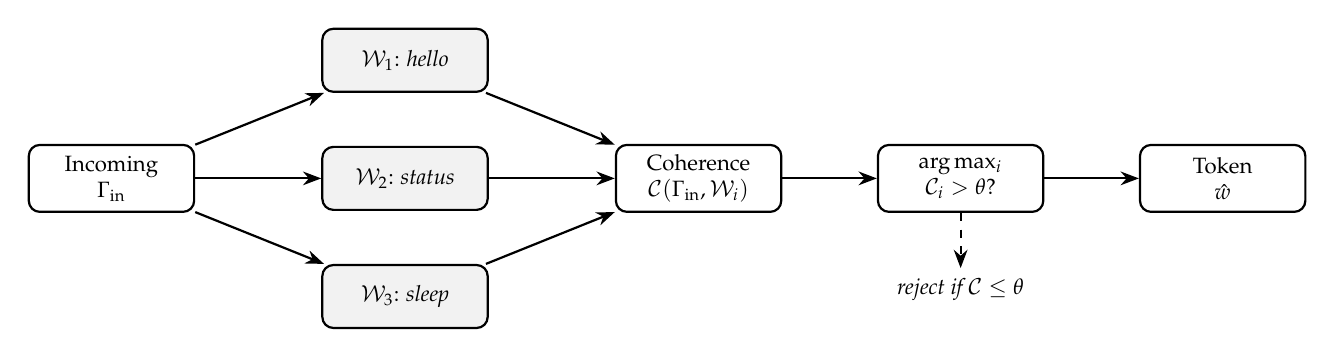
\begin{tikzpicture}[
    node distance=0.7cm and 1.1cm,
    every node/.style={font=\footnotesize},
    box/.style={rectangle, draw, thick, rounded corners, align=center,
                minimum width=2.1cm, minimum height=0.85cm, fill=white},
    basin/.style={rectangle, draw, thick, rounded corners, align=center,
                  minimum width=2.1cm, minimum height=0.8cm, fill=gray!10},
    arr/.style={-{Stealth}, thick},
    darr/.style={-{Stealth}, thick, dashed}
]
\node[box]   (gamma) {Incoming\\$\Gamma_{\mathrm{in}}$};

\node[basin, right=1.6cm of gamma, yshift=1.5cm]  (w1) {$\mathcal{W}_1$: \textit{hello}};
\node[basin, right=1.6cm of gamma]                  (w2) {$\mathcal{W}_2$: \textit{status}};
\node[basin, right=1.6cm of gamma, yshift=-1.5cm] (w3) {$\mathcal{W}_3$: \textit{sleep}};

\node[box, right=1.6cm of w2] (coh) {Coherence\\$\mathcal{C}(\Gamma_{\mathrm{in}},\mathcal{W}_i)$};
\node[box, right=1.2cm of coh] (argmax) {$\arg\max_i$\\$\mathcal{C}_i > \theta$?};
\node[box, right=1.2cm of argmax] (out) {Token\\$\hat{w}$};

\draw[arr] (gamma) -- (w1);
\draw[arr] (gamma) -- (w2);
\draw[arr] (gamma) -- (w3);
\draw[arr] (w1) -- (coh);
\draw[arr] (w2) -- (coh);
\draw[arr] (w3) -- (coh);
\draw[arr] (coh) -- (argmax);
\draw[arr] (argmax) -- (out);
\draw[-{Stealth}, thick, dashed] (argmax.south) -- ++(0,-0.7) node[below, font=\footnotesize\itshape]{reject if $\mathcal{C} \leq \theta$};
\end{tikzpicture}
\caption{Trajectory resonance recognition. The incoming trajectory $\Gamma_{\mathrm{in}}$ is compared against all stored word basins by the DTW coherence functional \eqref{eq:dtw}. Recognition collapses onto the basin with maximal coherence exceeding threshold $\theta$; trajectories with no basin above threshold are rejected. No classifier, no softmax: recognition is geometric collapse.}
\label{fig:recognition}
\end{figure}

\subsection{Trajectory Equivalence Across Modalities}

The trajectory formulation extends the prosodic equivalence of Section~5 into the temporal domain. A sequence of Hyperbionic text tokens $\{T_i\}$ with parameter vectors $\{p_i\}$ defines a discrete path in typographic parameter space:

\begin{equation}
\Gamma_{\mathrm{text}} = \{p_i\}_{i=1}^N.
\label{eq:Gtext}
\end{equation}

The equivalence \eqref{eq:equiv} then extends to trajectories:

\begin{equation}
\Gamma_{\mathrm{audio}} \;\sim\; \Gamma_{\mathrm{mem}} \;\sim\; \Gamma_{\mathrm{text}},
\label{eq:trajequiv}
\end{equation}

where equivalence is defined by preservation of prosodic invariants under projection. Speech-to-text is the operation $\Gamma_{\mathrm{audio}} \to \Gamma_{\mathrm{text}}$; text-to-speech is its inverse. Both are instances of trajectory reconstruction across modalities.


\section{From Salience Packets to Modal Trajectories}

The measurement operator $\mathcal{M}$, as previously defined, presents prosody as a direct mapping from waveform to vector. In practice, this mapping factors through a more primitive layer: a stream of discrete acoustic events. These events form the true substrate of the system, from which both statistical summaries and trajectories are derived. Formalizing this intermediate layer clarifies why the vector is not the fundamental object of the system, and motivates the trajectory representation as a natural consequence of event-based sampling rather than an additional design choice.

\subsection{The Salience Packet as Fundamental Unit}

The Marine processor does not sample the waveform uniformly. It samples \emph{events}: local maxima of the signal that exceed the clip threshold and satisfy the period validity gate. Each detected peak emits a \emph{salience packet}

\begin{equation}
\mathcal{P}_k = \bigl(j_p(k),\; j_a(k),\; h(k),\; s(k),\; E(k),\; t_k\bigr),
\label{eq:packet}
\end{equation}

where $j_p(k)$ is period jitter, $j_a(k)$ is amplitude jitter, $h(k)$ is harmonic alignment, $s(k)$ is the salience score, $E(k) = a_k^2$ is local peak energy, and $t_k$ is the sample index of the peak. The full output of the processor on a waveform segment is the ordered packet stream

\begin{equation}
u(t) \;\longrightarrow\; \{\mathcal{P}_k\}_{k=1}^N.
\label{eq:stream}
\end{equation}

The packet stream can equivalently be viewed as a discrete measure over event time:
\begin{equation}
\mu_u = \sum_{k=1}^N \delta_{t_k} \cdot \mathcal{P}_k,
\label{eq:measure}
\end{equation}
where $\delta_{t_k}$ is a Dirac mass at peak time $t_k$ and $\mathcal{P}_k$ is the associated packet value. Under this representation, the prosodic vector $\mathcal{M}(u) = \mathcal{A}(\mu_u)$ is a moment functional on $\mu_u$, and the trajectory $\Gamma = \{Z_\alpha(t_k)\}$ is the pushforward of $\mu_u$ under the quantization map $Q \circ \phi$. Aggregation and trajectory construction are therefore not two separate operations but two different functionals on the same underlying measure.

This event-based representation has three properties that distinguish it from uniform sampling. It is \emph{sparse}: packets are emitted only at peaks, so the stream has $N \ll T \cdot f_s$ elements for a waveform of duration $T$. It is \emph{physically grounded}: every component of $\mathcal{P}_k$ is a measured invariant of the signal, not a learned abstraction. And it is \emph{approximately rate-invariant}: because peaks are detected by local comparison rather than by absolute time index, two recordings of the same utterance at different speaking rates produce packet streams with similar jitter profiles but different lengths, which is exactly the structure that the DTW coherence functional in Section~7 is designed to exploit.

The prosodic vector $\mathcal{M}(u)$ defined in equation~\eqref{eq:Mvec} is now revealed as an \emph{aggregation} of the packet stream rather than a direct measurement:

\begin{equation}
\mathcal{M}(u) = \mathcal{A}\bigl(\{\mathcal{P}_k\}_{k=1}^N\bigr),
\label{eq:agg}
\end{equation}

where $\mathcal{A}$ computes the component-wise statistics (means, standard deviations, density, energy mean) defined in \eqref{eq:Mvec}. The two-stage chain is then

\begin{equation}
u(t)
\;\xrightarrow{\;\text{peak detection}\;}
\{\mathcal{P}_k\}
\;\xrightarrow{\;\mathcal{A}\;}
\mathcal{M}(u)
\;\xrightarrow{\;Q\;}
Z_\alpha \in \mathbb{Z}_{Q8.8}^8,
\label{eq:fullchain}
\end{equation}

making explicit that the packet stream is the primary object and the prosodic vector is a secondary, aggregate summary.

\subsection{Packet-to-Modal Projection}

The aggregation route \eqref{eq:agg} collapses temporal information: a vector $\mathcal{M}(u)$ contains no record of \emph{when} within the utterance each packet was emitted. For identity and emotion classification this may be acceptable, but for trajectory-based speech recognition it is not. The alternative is to project each packet individually into a modal coordinate:

\begin{equation}
Z_\alpha(t_k) = Q\bigl(\phi(\mathcal{P}_k)\bigr) \in \mathbb{Z}_{Q8.8}^8,
\label{eq:perpacket}
\end{equation}

where $\phi : \mathcal{P}_k \mapsto \mathbb{R}^8$ selects and possibly augments the packet components. A natural choice includes the six packet fields plus two local-variation terms:

\begin{equation}
\phi(\mathcal{P}_k) = \bigl(j_p(k),\; j_a(k),\; h(k),\; s(k),\; \rho(k),\; E(k),\; \Delta j_p(k),\; \Delta j_a(k)\bigr),
\label{eq:phi}
\end{equation}

where $\rho(k)$ is the instantaneous peak density estimated in a short window around $t_k$, and $\Delta j_p(k) = j_p(k) - j_p(k-1)$, $\Delta j_a(k) = j_a(k) - j_a(k-1)$ are first differences capturing local acceleration of jitter. The per-packet projection \eqref{eq:perpacket} produces a sequence of modal vectors indexed by peak time, from which the trajectory $\Gamma = \{Z_\alpha(t_k)\}_{k=1}^N$ is directly obtained. The three-level hierarchy is then

\begin{align}
\text{Local (event physics):} \quad &\mathcal{P}_k, \notag\\
\text{Global (statistical identity):} \quad &\mathcal{M}(u) = \mathcal{A}(\{\mathcal{P}_k\}), \label{eq:hierarchy}\\
\text{Temporal (trajectory meaning):} \quad &\Gamma = \{Z_\alpha(t_k)\}_{k=1}^N. \notag
\end{align}

All three representations derive from the same packet stream. They are not competing descriptions but projections of the packet stream onto different summary statistics.

\subsection{The SalienceMarker Enumeration as Topological Signal}

The Marine processor does not emit only packets. Its output type is the enumeration

\begin{equation}
\mathrm{SalienceMarker} \in \{\mathrm{Peak}(\mathcal{P}_k),\; \mathrm{Fracture},\; \mathrm{Noise},\; \mathrm{Insufficient}\},
\label{eq:marker}
\end{equation}

where $\mathrm{Fracture}$ marks silence or a gap in the signal (inter-peak period exceeding the validity gate), $\mathrm{Noise}$ marks a region of high-amplitude aperiodic signal (energy above the clip threshold but no coherent peaks), and $\mathrm{Insufficient}$ marks a region where the processor has not yet warmed up. This enumeration introduces topological structure into the signal: rather than a continuous function, the processor produces a partition of the timeline into structured regions (voiced, voiced-unstable), boundaries (fractures between voiced regions), and noise fields.

The Fracture marker is particularly important for the trajectory architecture. A trajectory $\Gamma$ is a sequence of modal coordinates at peak times; a Fracture between two peaks creates a gap in the sequence that is not filled by interpolation. Word basins $\mathcal{W}_i$ therefore naturally encode the silence structure of the corresponding utterance, and the DTW alignment path $\pi$ in equation~\eqref{eq:dtw} must skip over Fracture gaps in both the query and the stored basin consistently. The Fracture marker therefore induces a canonical decomposition of any trajectory into voiced components separated by silence boundaries:
\begin{equation}
\Gamma = \bigsqcup_{m} \Gamma_m,
\label{eq:decomp}
\end{equation}
where each $\Gamma_m$ is a connected voiced segment and $\sqcup$ denotes disjoint union. DTW alignment is restricted to pairs within the same component; TARTAN tiles inherit this segmentation, with boundary flags $b_{\ell,j}$ propagating the Fracture structure up the hierarchy. In the Hyperbionic rendering, Fracture events correspond to typographic white space: the absence of prosodic transformation between adjacent tokens is itself a prosodic signal. The system thus maintains a clean distinction between two kinds of absence: silence removes points from $\Gamma$ entirely (a topological gap in the trajectory), while low salience down-weights existing points in $\mathcal{C}$ without removing them (a geometric thinning of the trajectory). Conflating these two would misclassify quiet expressive passages as silence; the Fracture marker prevents this by requiring energy to fall below the clip threshold, not merely for salience to be low.

\section{A Real Trajectory Space and TARTAN Multiscale Tiling}

\noindent\textit{This section establishes the real geometric structure of trajectory space and introduces a multiscale organization required for stability. Raw trajectories are sensitive to local perturbations; TARTAN constructs a hierarchy that preserves global structure while isolating local noise, allowing recognition to operate at the appropriate scale. Its role is not compression but stabilization.}


The trajectory representation $\Gamma = \{Z_\alpha(t_k)\}$ is powerful but fragile in a specific way: a small perturbation in a single packet---a spurious peak, a momentary noise spike---can shift the trajectory locally and degrade DTW coherence. A robust architecture requires a multiscale organization that separates global word shape from local packet noise.

\subsection{The Real Trajectory Space}

Before introducing the multiscale structure, it is useful to state the trajectory space precisely. After rescaling the fixed-point vectors to real values, each modal coordinate is an element of $V = \mathbb{R}^8$, and the inner product is the ordinary real dot product

\begin{equation}
\langle Z, Z' \rangle = \sum_{i=1}^{8} Z_i Z'_i.
\label{eq:ip}
\end{equation}

No imaginary components are required.

\begin{proposition}[Geometric Phase Representation]
Let $\Gamma \subset \mathbb{R}^8$ be a trajectory in modal space $V$. All phase-dependent interference effects are representable as geometric relations on $\Gamma$ under the real inner product structure of $V$. No complex extension is required.
\end{proposition}

Phase mismatch corresponds to trajectory divergence under alignment: two trajectories that would destructively interfere in a complex-exponential model appear as misaligned paths under the DTW coherence functional, yielding low or negative $\mathcal{C}$. Phase-like structure is represented geometrically by the direction of trajectory movement through modal space, not by imaginary coefficients. The space of finite trajectories of any length is $\mathcal{T} = \bigcup_{N \geq 1} V^N$, and the normalized coherence between two trajectories under an alignment path $\pi$ is

\begin{equation}
\mathcal{C}(\Gamma, \Gamma') = \frac{1}{|\pi|} \sum_{(k,\ell) \in \pi} \frac{\langle Z_\alpha(t_k), Z'_\alpha(t_\ell) \rangle}{\|Z_\alpha(t_k)\| \cdot \|Z'_\alpha(t_\ell)\| + \varepsilon},
\label{eq:Cnorm}
\end{equation}

where $\varepsilon > 0$ prevents division by zero for silent or near-zero packets. The coherence is in $[-1, 1]$, with $\mathcal{C} = 1$ indicating perfect alignment and $\mathcal{C} \leq 0$ indicating destructive interference: the two trajectories are moving in incompatible directions in modal space at the aligned time steps.

\subsection{TARTAN: Trajectory-Aware Recursive Tiling with Annotated Noise}

A raw trajectory $\Gamma = \{Z_\alpha(t_k)\}_{k=1}^N$ operates at the finest temporal scale---one modal vector per detected peak. For recognition, retrieval, and storage, it is advantageous to organize this fine-grained sequence into a hierarchy of coarser approximations. The TARTAN framework provides this organization.

TARTAN maps a raw trajectory to a sequence of tiled approximations at increasing coarseness levels:

\begin{equation}
\Gamma \;\longrightarrow\; \mathcal{T}_0(\Gamma),\; \mathcal{T}_1(\Gamma),\; \ldots,\; \mathcal{T}_L(\Gamma),
\label{eq:tartan}
\end{equation}

where $\mathcal{T}_0(\Gamma) = \Gamma$ is the original packet-level trajectory and each $\mathcal{T}_{\ell+1}$ is obtained by recursively tiling $\mathcal{T}_\ell$: partitioning it into non-overlapping segments and replacing each segment with a local summary tile

\begin{equation}
\tau_{\ell,j} = \bigl(\bar{Z}_{\ell,j},\; \Sigma_{\ell,j},\; \eta_{\ell,j},\; b_{\ell,j}\bigr),
\label{eq:tile}
\end{equation}

where $\bar{Z}_{\ell,j}$ is the mean modal vector over the segment, $\Sigma_{\ell,j}$ is a scalar or diagonal measure of local variance, $\eta_{\ell,j}$ is an annotated noise estimate (derived from the Noise markers in the SalienceMarker stream), and $b_{\ell,j} \in \{0, 1\}$ is a boundary flag marking whether a Fracture occurred within the segment.

The boundary flag is the key innovation: by propagating Fracture information up the tiling hierarchy, TARTAN ensures that silence structure is preserved at every scale. A coarse tile spanning a silence boundary is annotated as such, so that alignment at the coarse level does not inadvertently match voiced content across a silence gap.

Multiscale recognition proceeds by computing a weighted coherence across levels:

\begin{equation}
\mathcal{C}_{\mathrm{TARTAN}}(\Gamma, \Gamma') = \sum_{\ell=0}^{L} w_\ell\, \mathcal{C}\bigl(\mathcal{T}_\ell(\Gamma),\; \mathcal{T}_\ell(\Gamma')\bigr),
\label{eq:Ctartan}
\end{equation}

where the weights satisfy
\begin{equation}
\sum_{\ell=0}^{L} w_\ell = 1, \qquad w_0 \geq w_1 \geq \cdots \geq w_L > 0,
\label{eq:tartanweights}
\end{equation}
enforcing coarse-to-fine dominance. This normalization ensures that $\mathcal{C}_{\mathrm{TARTAN}} \in [-1, 1]$ whenever each level coherence is normalized, and the monotone decrease prevents fine-level packet noise from destabilizing recognition. At coarse levels the system detects global word shape; at fine levels it verifies local prosodic microstructure. Recognition requires $\mathcal{C}_{\mathrm{TARTAN}}(\Gamma, \mathcal{W}_i) > \theta$ for a stored word basin $\mathcal{W}_i$.

\subsection{The Complete Equivalence}

With all components in place, the full processing pipeline is

\begin{equation}
u(t)
\;\xrightarrow{\;\text{Marine}\;}
\{\mathcal{P}_k\}
\;\xrightarrow{\;\phi, Q\;}
\{Z_\alpha(t_k)\}
\;\xrightarrow{\;\text{TARTAN}\;}
\{\mathcal{T}_\ell(\Gamma)\}_{\ell=0}^{L},
\label{eq:pipeline}
\end{equation}

and the Hyperbionic visual trajectory $\Gamma_{\mathrm{text}} = \{p_i\}$ is a rendering of the same packet-derived structure into typographic parameter space. The equivalence \eqref{eq:trajequiv} therefore extends to include the TARTAN representation:

\begin{equation}
\Gamma_{\mathrm{audio}} \;\sim\; \Gamma_{\mathrm{mem}} \;\sim\; \Gamma_{\mathrm{tartan}} \;\sim\; \Gamma_{\mathrm{text}},
\label{eq:fullequiv}
\end{equation}

where equivalence is preservation of prosodic invariants under admissible projection at each stage. The four components of the system have distinct roles that are now precisely delineated: Marine performs event extraction, MEM$|$8 provides modal storage of quantized packet coordinates, TARTAN organizes trajectories into multiscale tiles that are robust to local packet noise, and Hyperbionic Reading renders the same trajectory structure as a visual field. None of these roles overlaps; each is a necessary stage in the pipeline from acoustic signal to visual prosody.

\begin{figure}[p]
\centering
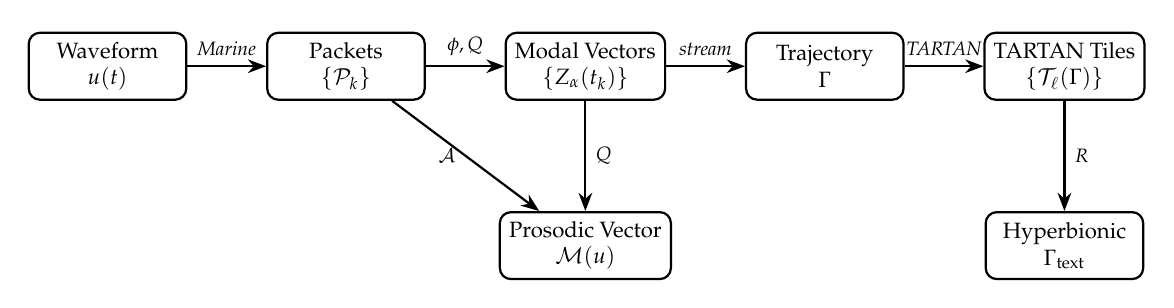
\begin{tikzpicture}[
    node distance=0.7cm and 1.0cm,
    every node/.style={font=\footnotesize},
    box/.style={rectangle, draw, thick, rounded corners, align=center,
                minimum width=2.0cm, minimum height=0.85cm, fill=white},
    arr/.style={-{Stealth}, thick},
    label/.style={font=\scriptsize\itshape, midway, above}
]
\node[box] (audio)   {Waveform\\$u(t)$};
\node[box, right=of audio]  (pkts)  {Packets\\$\{\mathcal{P}_k\}$};
\node[box, right=of pkts]   (modal) {Modal Vectors\\$\{Z_\alpha(t_k)\}$};
\node[box, right=of modal]  (traj)  {Trajectory\\$\Gamma$};
\node[box, right=of traj]   (tartan){TARTAN Tiles\\$\{\mathcal{T}_\ell(\Gamma)\}$};

\node[box, below=1.4cm of modal] (mvec) {Prosodic Vector\\$\mathcal{M}(u)$};
\node[box, below=1.4cm of tartan] (hyper) {Hyperbionic\\$\Gamma_{\mathrm{text}}$};

\draw[arr] (audio)  -- node[label]{Marine} (pkts);
\draw[arr] (pkts)   -- node[label]{$\phi,Q$} (modal);
\draw[arr] (modal)  -- node[label]{stream} (traj);
\draw[arr] (traj)   -- node[label]{TARTAN} (tartan);

\draw[arr] (pkts)   -- node[font=\scriptsize\itshape, left]{$\mathcal{A}$} (mvec);
\draw[arr] (modal)  -- node[font=\scriptsize\itshape, right]{$Q$} (mvec);
\draw[arr] (tartan) -- node[font=\scriptsize\itshape, right]{$R$} (hyper);
\end{tikzpicture}
\caption{Full processing pipeline. The waveform $u(t)$ is converted by the Marine processor into a sparse packet stream $\{\mathcal{P}_k\}$. Per-packet projection $\phi$ followed by quantization $Q$ yields modal vectors; their sequence is the trajectory $\Gamma$. TARTAN organizes $\Gamma$ into a multiscale tile hierarchy. Aggregation $\mathcal{A}$ collapses the packet stream to the prosodic vector $\mathcal{M}(u)$ (statistical identity path). The Hyperbionic rendering operator $R$ projects the tiled trajectory into the visual field.}
\label{fig:pipeline}
\end{figure}


\section{Reconstruction and Cue-Based Retrieval}

The bidirectionality of the framework raises a question about information recovery. Given a Hyperbionic rendering $R(g, p)$, can the original prosodic structure be recovered? The answer depends on which components of $p$ are preserved under rendering and which are collapsed in the visual output.

For the core parameters in Table~\ref{tab:mapping}, the mapping is injective in principle: given a rendered glyph and knowledge of the rendering operator $R$, the parameter vector $p$ can be extracted by inverting the visual-to-parameter correspondences. In practice, quantization and rendering resolution introduce information loss, but the loss is bounded by the same constraints that govern the admissibility of $R$: a rendering that is legible is one that preserves enough visual variation to make the parameter vector recoverable.

This recovery structure corresponds to what Tulving identified as \emph{synergistic ecphory}: the process by which a partial retrieval cue, combined with stored engram information, produces a recollective state that neither the cue nor the engram alone determines~\cite{Tulving1982}. Hyperbionic text functions as a structured cue set for prosodic reconstruction. The rendered glyph is the cue; the stored prosodic vector (or, in the MEM$|$8 case, the modal lattice coordinate) is the engram; and the reconstructed acoustic impression is their joint product. The full reconstruction chain is

\begin{equation}
R(g, p) \;\xrightarrow{\;R^{-1}\;}\; p \;\xrightarrow{\;Q^{-1}\;}\; \mathcal{M}(u) \;\xrightarrow{\;\text{synthesis}\;}\; \hat{u}(t),
\label{eq:recon}
\end{equation}

where $\hat{u}(t)$ is a reconstructed waveform consistent with the recovered prosodic vector. This is not lossless reconstruction of the original waveform---the measurement operator $\mathcal{M}$ is many-to-one, and distinct waveforms with the same prosodic vector are indistinguishable at the level of \eqref{eq:Mvec}---but it is reconstruction of prosodic structure, which is precisely the structure that plain text discards and Hyperbionic rendering preserves.

\section{Constraints and Stability}

The expressive power of the Hyperbionic system must be bounded to remain usable. Without constraints, the parameter space $\mathbb{R}^m$ allows mappings that render text unreadable---glyphs too small to resolve, rotations that invert letterforms, displacements that destroy word boundaries.

Before developing the formal constraints, it is useful to note that the admissibility problem has a precise analogue in the audio domain. Standard lossy codecs (MP3, AAC) apply a psychoacoustic masking model: when a loud transient such as a snare hit occurs immediately before a quiet signal such as a vocal breath, the algorithm discards the quiet signal on the grounds that the loud event masks it. This produces what audio engineers call \emph{spectral fracturing}: metallic ringing, temporal smearing, and pre-echo artifacts that the auditory system registers subconsciously even when the conscious mind cannot identify them. The computational load of repairing the fractured signal blunts emotional impact.

Spectral fracturing is, in the framework of this paper, a pathological aggregation: a codec that discards masked signal components is a system that factors through a lossy version of $\mathcal{A}$, and by the Aggregation Impossibility Proposition the resulting representation cannot recover expressive coherence $\chi$. What is destroyed is precisely the structured microdynamic jitter that carries the emotional carrier wave---the subtle harmonic weight and temporal micro-variation of a human performance that cannot be reconstructed from amplitude and spectral envelope alone. Hyperbionic rendering must avoid the typographic analogue of spectral fracturing: transformations that preserve nominal glyph structure while destroying the coherence required for perceptual integration. An admissible rendering is one that neither collapses prosodic distinctions nor introduces visual artifacts that impose a reconstruction burden on the reader analogous to the cognitive load of a fractured audio signal. The admissibility constraints introduced informally in Section~4 can be stated precisely.

Define the \emph{perceptual validity region} as the set of parameter vectors $p_i$ such that the rendered glyph $R(g_i, p_i)$ is legible at normal reading distance and reading speed. This region is bounded: there exist maximum and minimum values for each parameter beyond which legibility fails. Within this region, the constraint energy

\begin{equation}
C[p] = \int_{\mathcal{M}} \left(\alpha\, \theta(x)^2 + \beta\, S(x)^2 + \gamma\, \xi(x)^2\right) d\mu(x)
\label{eq:Cp}
\end{equation}

---where $\theta$ measures misalignment between the rendering trajectory and the salience gradient, $S$ measures uncertainty in parameter values, and $\xi$ measures rotational instability in the visual field---is bounded above by a legibility threshold $C_{\max}$. Admissible renderings satisfy $C[p] \leq C_{\max}$.

The legibility constraint has a further consequence: it implies that Hyperbionic rendering operates on a low-dimensional admissible manifold within the full parameter space. Not all combinations of the parameters in \eqref{eq:pi} are jointly admissible; the constraints couple the parameters and restrict the system to a structured subset of $\mathbb{R}^m$. This is the typographic analogue of the biological prior in cognitive trajectory models: the system does not search the full parameter space uniformly but is confined by legibility and stability constraints to a lower-dimensional structured region.

The perceptual weights $w_i$ in the $G$-metric are not universal but listener-variable. A relevant empirical observation is that audiometric studies have reported that women, on average, exhibit approximately 2 dB greater sensitivity than men across frequency ranges, a difference attributed to evolutionary pressures related to detecting the high-frequency cues of infant distress. If this differential sensitivity is real and of the reported magnitude, it has a direct consequence for spectral fracturing: compression artifacts that fall below the conscious detection threshold of a less sensitive auditory system may register supra-threshold for a more sensitive one, imposing a subconscious cognitive load on the listener that blunts emotional impact. In the framework of this paper, this corresponds to listener-specific $G$-metrics with higher weights on the dimensions most affected by compression artifacts---temporal fine structure and high-frequency harmonic content. A Hyperbionic rendering system that aims to preserve emotional impact across a diverse listener population must therefore parameterize $G$ as a function of the target perceptual profile, not treat it as a fixed universal constant. The claim about 2 dB differential sensitivity is taken from existing discourse on this topic and should be understood as an empirical hypothesis requiring controlled audiometric validation rather than an established universal constant; the structural point about listener-variable $G$-metrics holds independently of the specific magnitude. The system must therefore treat $G$ as a parameterized perceptual model rather than a fixed metric, adapting the weighting structure to the sensitivity profile of the target observer.


\section{Implementation: The Marine Processor as $\mathcal{M}$ in Practice}

The measurement operator $\mathcal{M}$ defined in Section~2 is not merely a formal object. It has a concrete, running implementation in the Marine processor, a Rust library designed for $O(1)$ per-sample operation. Examining the implementation reveals three places where the formal definition and the executable code diverge in instructive ways, and one where the implementation makes a stronger architectural commitment than the formalism requires.

\subsection{Exponential Moving Average versus Window Mean}

The formal definition of period jitter uses sample means: $j_p(k) = |\Delta t_k - \overline{\Delta t}| / \overline{\Delta t}$, where $\overline{\Delta t}$ is the mean inter-peak interval over all observed peaks. This is clean mathematically but impractical for real-time processing, since computing the sample mean requires storing all past periods and updating a running sum---operations that are $O(N)$ in memory if not time.

The implementation replaces the sample mean with an exponential moving average (EMA). Let $\mu_k$ denote the EMA of inter-peak periods after the $k$-th peak. The update rule is

\begin{equation}
\mu_k = \alpha_p \cdot \Delta t_k + (1 - \alpha_p) \cdot \mu_{k-1},
\label{eq:ema}
\end{equation}

where $\alpha_p \in (0,1)$ is the EMA smoothing coefficient configured at initialization. Jitter is then computed as $j_p(k) = |\Delta t_k - \mu_{k-1}| / \mu_{k-1}$, using the previous EMA value as the reference rather than the global mean. An identical EMA $\mu^a_k$ tracks peak amplitudes for the amplitude jitter computation.

The classical definition of jitter assumes a stationary reference distribution. This assumption is violated in natural speech, where fundamental frequency drifts continuously over time. The EMA formulation replaces a global reference with a locally adaptive one, allowing the system to track prosodic intent rather than penalize it as deviation. The substitution is therefore not an optimization but a correction to the measurement model itself: the formal definition in equation~\eqref{eq:Mvec} should be read as using a weighted mean with exponential decay rather than a uniform sample mean. A speaker who gradually lowers their pitch will show low EMA-based jitter throughout, correctly identifying the signal as locally periodic despite global drift; the sample-mean version would misclassify the drift as instability.

The EMA also implements the warmup condition implicitly. The processor exposes an \texttt{is\_warmed\_up()} predicate that returns true only when at least three peaks have been detected and the EMA has received enough updates to be reliable. Formally, this means that $\mathcal{M}(u)$ is a partial function: it is undefined on waveforms too short to contain at least three peaks satisfying the minimum period constraint. The sliding window $\gamma(t) = \mathcal{M}(u\!\upharpoonright_{[t-\Delta, t]})$ introduced in Section~7 therefore requires a window width $\Delta$ satisfying

\begin{equation}
\Delta \geq \frac{3}{f_0},
\label{eq:warmup}
\end{equation}

where $f_0$ is the fundamental frequency of the signal. For speech at 100--300 Hz, this constrains $\Delta \geq 10$--$30$ milliseconds---a natural lower bound that the implementation enforces implicitly through the warmup predicate.

\subsection{The Harmonic Coherence Placeholder}

The formal vector \eqref{eq:Mvec} includes a harmonic coherence component $h$ measuring the degree of periodic regularity in the voiced signal. In the current implementation, this component is hardcoded to $h = 1.0$ with a comment marking it as a TODO item: \enquote{Harmonic score (simplified -- TODO: FFT-based detection). For now, assume voiced content.}

This means the implementation currently computes a seven-dimensional effective vector, not an eight-dimensional one. The eighth dimension---harmonic coherence---is present structurally but carries no information. The salience score $s = 1/(1 + j_p + j_a)$ is consequently computed from jitter alone, without any contribution from spectral periodicity. Signals with strong harmonic structure (sustained vowels) and signals with weak harmonic structure (fricatives, noise) receive the same $h$ value and are distinguished only by their jitter profiles.

The intended extension is FFT-based harmonic detection: computing the ratio of energy at the fundamental frequency and its harmonics to total signal energy, which gives a value in $[0,1]$ that approaches 1 for purely periodic signals and 0 for white noise. Formally,

\begin{equation}
h = \frac{\sum_{k=1}^{K} |U(k f_0)|^2}{\int_0^{f_s/2} |U(f)|^2\, df},
\label{eq:h}
\end{equation}

where $U(f)$ is the discrete Fourier transform of a windowed segment of $u(t)$, $f_0$ is the estimated fundamental frequency, and $K$ is the number of harmonics included. This computation is $O(N \log N)$ per window rather than $O(1)$ per sample, which is why it has not yet been integrated: it would require a hybrid architecture in which the peak-based $O(1)$ processor feeds a periodic FFT-based harmonic estimator operating on a longer lookback buffer.

The formal framework anticipates this extension naturally. The measurement operator $\mathcal{M}$ is defined abstractly as a map to $\mathbb{R}^n$; the specific components are a concrete instance, not a structural constraint. Adding a genuinely computed $h$ component does not change the architecture of the Hyperbionic system---the equivalence \eqref{eq:equiv} holds for any prosodic parameter vector, regardless of dimensionality---but it does change the information content of the modal coordinate $Z_\alpha$ and therefore the discriminative power of the trajectory resonance recognizer. Utterances that are currently indistinguishable (same jitter profiles, different harmonic structure) would become distinguishable once $h$ is measured rather than assumed. Until this component is implemented, the system operates in a reduced discriminative regime in which periodicity is inferred indirectly through jitter rather than measured explicitly. This is a structural limitation of the current implementation, not merely an engineering detail.

\section{Operational Constraints and Real-Time Geometry}

The Marine processor enforces two further constraints that have formal analogues in the measurement operator's domain of definition: a period validity gate and a clip threshold.

\subsection{Period Validity Gate}

The processor accepts a peak contribution only when the inter-peak period falls within a configurable range $[\texttt{min\_period}, \texttt{max\_period}]$ specified in samples. This gate serves two purposes: it excludes spurious detections (very short periods corresponding to noise spikes) and it excludes silence gaps (very long periods corresponding to pauses between utterances). Formally, let $f_s$ denote the sample rate. The gate defines an admissible frequency range

\begin{equation}
f_{\min} = \frac{f_s}{\texttt{max\_period}}, \qquad f_{\max} = \frac{f_s}{\texttt{min\_period}},
\label{eq:frange}
\end{equation}

and the measurement operator is defined only on signal segments whose instantaneous fundamental frequency lies within $[f_{\min}, f_{\max}]$. For the default speech configuration at 22050 Hz, typical values confine the operator to voiced fundamental frequencies in the speech range, rejecting both subsonic artifacts and aliased high-frequency noise.

The period gate has a geometric interpretation in trajectory space. A trajectory $\Gamma = \{Z_\alpha(t_k)\}$ is defined only at time steps where a valid peak is detected within the admissible period range. At time steps where the signal is silent, unvoiced, or outside the frequency range, the trajectory is undefined---the point is simply absent from the sequence. This means that word basins $\mathcal{W}_i$ are sparse trajectories: sequences of modal coordinates at the times of valid peaks, with gaps corresponding to unvoiced or silent intervals. The DTW coherence functional \eqref{eq:dtw} must be understood as aligning sparse sequences, not dense time series, which the standard DTW algorithm handles naturally through its admissible alignment path constraint.

\subsection{Clip Threshold as a Pre-Gate}

Before any peak detection is attempted, the processor applies a clip threshold: samples with absolute value below \texttt{clip\_threshold} are ignored entirely, bypassing even the peak detection logic. This is a pre-gate that defines the silence floor of the system.

Formally, let $\varepsilon_{\mathrm{clip}} > 0$ denote the clip threshold. The effective input to $\mathcal{M}$ is not $u(t)$ itself but the gated signal

\begin{equation}
u_\varepsilon(t) = \begin{cases} u(t) & \text{if } |u(t)| \geq \varepsilon_{\mathrm{clip}}, \\ 0 & \text{otherwise.} \end{cases}
\label{eq:gate}
\end{equation}

The measurement operator $\mathcal{M}$ acts on $u_\varepsilon$, not on $u$. This means that very quiet passages---below the noise floor of the recording environment---contribute no peaks and no trajectory points. The clip threshold is therefore the operational definition of silence in the Marine framework: a continuous segment on which $u(t)$ lies entirely below $\varepsilon_{\mathrm{clip}}$ produces no output from $\mathcal{M}$, and its absence from the trajectory is the signal that a silence or unvoiced interval has occurred.

In the Hyperbionic context, this gating has a direct typographic correlate. Tokens in a transcript that correspond to silent intervals---pauses, breaths, hesitations---receive no prosodic parameter vector from $\mathcal{M}$, and so their Hyperbionic rendering falls back to the default glyph $R(g_i, \mathbf{0})$: unstyled, unmodified text. Silence becomes the absence of typographic transformation, which is the correct rendering: a pause in speech is marked in Hyperbionic text by the surrounding white space, not by any active visual property of the adjacent glyphs.


\section{Beyond the Audible-Stable Regime: Haptic Extension and Expressive Deviation}

\noindent\textit{This section removes two simplifying assumptions of the preceding framework: that all relevant structure lies within the audible band, and that deviation from periodicity is noise. Both assumptions exclude meaningful signal. The extensions introduced here incorporate sub-audible somatic structure and reinterpret deviation as a carrier of intention, completing the invariant field.}


The formulation developed thus far assumes that prosodic structure is captured by stable periodic features within the audible frequency band. This assumption is both physically and perceptually incomplete in two orthogonal directions. First, acoustic signals below approximately 40 Hz are not primarily perceived auditorily but somatically, as vibration felt in the chest, body, and surrounding environment. Second, the salience formula $s = 1/(1 + \overline{j_p} + \overline{j_a})$ treats all jitter as degradation, which is correct for detecting synthetic or damaged signals but wrong for expressive performance, where controlled deviation is the carrier of meaning. What was previously classed as noise occupies exactly the dimensions where intention lives.

\subsection{Infrasound and the Haptic Channel}

The Marine configuration gates the measurement operator to an admissible frequency range $[f_{\min}, f_{\max}]$ corresponding to roughly 60--4000 Hz for speech. Signals below $\sim 40$ Hz are discarded. But low-frequency content below the auditory threshold is not absent from musical and environmental signals: the sub-bass of a bass guitar, the chest-felt pulse of a kick drum, the room pressure of a large acoustic space are all real physical quantities that carry structural information about the source and environment.

Let $u(t)$ be decomposed spectrally into
\begin{equation}
u(t) = u_{\mathrm{aud}}(t) + u_{\mathrm{infra}}(t),
\label{eq:decomp_freq}
\end{equation}
where $u_{\mathrm{infra}}$ contains components with instantaneous frequency $f < 40$ Hz. The current measurement operator $\mathcal{M}$ acts only on $u_{\mathrm{aud}}$. We define the extended measurement operator
\begin{equation}
\widetilde{\mathcal{M}}(u) = \bigl(\mathcal{M}(u_{\mathrm{aud}}),\; H(u_{\mathrm{infra}})\bigr),
\label{eq:Mtilde}
\end{equation}
where $H$ is a \emph{haptic measurement functional} extracting the low-frequency envelope:
\begin{equation}
H(u_{\mathrm{infra}}) = \bigl(A_{\mathrm{lf}},\; \sigma_{\mathrm{lf}},\; \nabla A_{\mathrm{lf}}\bigr).
\label{eq:H}
\end{equation}
Here $A_{\mathrm{lf}}$ is the low-frequency energy envelope, $\sigma_{\mathrm{lf}}$ its temporal variance, and $\nabla A_{\mathrm{lf}}$ its rate of change. These quantities encode perceived pressure, pulsation rate, and environmental resonance---the somatic correlates of musical bass.

The haptic channel is structurally distinct from the auditory channel in two respects. Perceptually, infrasound is field-like: it is felt across the whole body rather than localized in the auditory system, and the relevant spatial scale is the body or room rather than the cochlea. This means that in the Hyperbionic rendering, infrasound does not map to glyph-level deformation but to \emph{global layout modulation}---baseline drift, field-wide spacing variation, or background texture---reflecting the distributed rather than localized nature of somatic perception. Formally, the trajectory space extends to $V = \mathbb{R}^{8+3}$, with the three haptic dimensions decoupled from the $G$-metric of the auditory dimensions and requiring separate perceptual weighting.

\subsection{Structured Jitter as Expressive Signal}

Jitter, in the current framework, is defined as deviation from an exponentially weighted expected period. But this definition conflates two categorically different phenomena. Random jitter arises from measurement noise, imprecise articulation, or signal degradation: it has no temporal structure and carries no information beyond the degradation level. Structured jitter arises from intentional expressive modulation: vibrato in a sustained note is periodic jitter; groove in a rhythm section is timing jitter locked to a metrical grid; the roughness of a distorted guitar is amplitude jitter with a specific spectral signature. These are not corruptions of a periodic signal but features of it.

We decompose the observed jitter sequence $\{j(k)\}$ into two components:
\begin{equation}
j(k) = j_{\mathrm{rand}}(k) + j_{\mathrm{expr}}(k),
\label{eq:jdecomp}
\end{equation}
where $j_{\mathrm{rand}}$ is stochastic and carries no predictive structure, and $j_{\mathrm{expr}}$ is structured, reproducible, and carries expressive information.

\begin{definition}[Expressive Coherence]
Let $\{j(k)\}_{k=1}^N$ be a sequence of jitter measurements and $\{\hat{j}(k)\}$ a locally predicted sequence obtained by fitting a short-memory model to recent values. The \emph{expressive coherence} is
\begin{equation}
\chi = 1 - \frac{\mathrm{Var}\bigl(j(k) - \hat{j}(k)\bigr)}{\mathrm{Var}\bigl(j(k)\bigr)},
\label{eq:chi}
\end{equation}
with $\chi \in [0, 1]$: $\chi \approx 1$ when deviation follows a predictable pattern, $\chi \approx 0$ when deviation is indistinguishable from white noise.
\end{definition}

High $\chi$ at substantial $\overline{j}$ indicates expressive performance. Low $\chi$ at substantial $\overline{j}$ indicates damage or noise. Low $\chi$ at low $\overline{j}$ indicates a synthetic or mechanically regular signal. The original scalar salience $s$ cannot distinguish the first from the third of these cases when mean jitter happens to be comparable; the expressive coherence $\chi$ distinguishes all three.

We define a second salience axis
\begin{equation}
s_{\mathrm{expr}} = \chi \cdot (\overline{j_p} + \overline{j_a}),
\label{eq:sexpr}
\end{equation}
measuring the magnitude of structured deviation: it is large when jitter is both substantial and organized. The full salience representation is then two-dimensional:
\begin{equation}
\mathbf{s} = (s_{\mathrm{stable}},\; s_{\mathrm{expr}}),
\label{eq:s2d}
\end{equation}
where $s_{\mathrm{stable}} = s = 1/(1 + \overline{j_p} + \overline{j_a})$ is the existing periodicity salience and $s_{\mathrm{expr}}$ is the new expressive axis. Stable periodic signals maximize $s_{\mathrm{stable}}$; expressive signals maximize $s_{\mathrm{expr}}$; synthetic or damaged signals minimize both.

The two-dimensional salience space has an important application to the authentication of human performance. A human vocal performance is produced by a coupled physical system: lungs, diaphragm, vocal cords, resonant cavities, and neural motor control all constrain the jitter profile jointly. The resulting jitter is not random but structured by physiology---it lies near the constraint manifold of a biological dynamical system. We call this property \emph{biological coupling}: the jitter sequence is organized by a physical process that imposes internal consistency across time scales from milliseconds (glottal pulse variation) to seconds (respiratory cycle). Generative audio synthesis systems, by contrast, produce jitter by sampling from learned distributions over spectral and temporal features. The resulting jitter is \emph{decoupled}: it may match the marginal statistics of human jitter (mean, variance, spectral envelope) while failing to reproduce the coupled temporal structure. In the framework of this paper, biological coupling corresponds to high $\chi$ with a structured manifold, while decoupled synthetic jitter produces low $\chi$ despite superficially plausible amplitude and pitch.

\begin{proposition}[Biological Coupling Detectability]
Let $u_{\mathrm{human}}$ be a human vocal performance and $u_{\mathrm{synth}}$ a generative synthesis of the same utterance. If the synthesis system matches the aggregate statistics $\mathcal{M}(u_{\mathrm{human}}) \approx \mathcal{M}(u_{\mathrm{synth}})$ but does not model the physiological coupling of the human jitter process, then $\chi(u_{\mathrm{human}}) \gg \chi(u_{\mathrm{synth}})$ and the two signals are distinguishable by trajectory coherence even when indistinguishable by aggregate prosodic statistics.
\end{proposition}

This proposition provides the mathematical basis for biometric voice authentication via expressive coherence: the structured biological jitter of a human performance is not merely a stylistic feature but a physically grounded invariant that aggregate-matching synthesis cannot replicate without modeling the underlying physiology. This establishes a separation principle: synthesis systems that match marginal statistics but fail to reproduce coupled temporal structure remain distinguishable under trajectory-based metrics. A voice authentication system based on $\chi$ is therefore resistant to attacks that match spectral envelope, pitch contour, and mean jitter while lacking the physiological coupling that generates structured temporal coherence in human performance.

\begin{proposition}[Aggregation Information Loss]
The aggregation map $\mathcal{A}$ is not injective on trajectories: $\mathcal{A}(\Gamma_1) = \mathcal{A}(\Gamma_2)$ does not imply $\Gamma_1 = \Gamma_2$. Therefore any system that operates exclusively on $\mathcal{M}(u) = \mathcal{A}(\{\mathcal{P}_k\})$ cannot recover trajectory curvature or expressive coherence $\chi$.
\end{proposition}

\hyperemph{This is not a limitation of any particular model design but a general impossibility result for the class of representations that factor through $\mathcal{A}$.} Standard acoustic embedding systems, which map utterances to fixed-length vectors derived from averaged or pooled features, belong to this class. The trajectory-based architecture proposed here does not factor through $\mathcal{A}$, and so is not subject to this limitation.

\subsection{Reinterpretation of Annotated Noise in TARTAN}

Under the original formulation, the annotated noise field $\eta_{\ell,j}$ in each TARTAN tile records structured deviation to be tracked and, implicitly, suppressed or normalized away. The decomposition \eqref{eq:jdecomp} and the expressive coherence \eqref{eq:chi} permit a more discriminating treatment. Each tile is extended to
\begin{equation}
\tau_{\ell,j} = \bigl(\bar{Z}_{\ell,j},\; \Sigma_{\ell,j},\; \eta_{\ell,j},\; \chi_{\ell,j},\; b_{\ell,j}\bigr),
\label{eq:tileext}
\end{equation}
where $\chi_{\ell,j}$ is the expressive coherence computed over the packets within tile $(\ell, j)$. The noise field $\eta_{\ell,j}$ and coherence $\chi_{\ell,j}$ together classify tile content:
\begin{align}
\eta \approx 0,\; \chi \approx 0 &\;\Rightarrow\; \text{silence or highly stable signal,} \notag\\
\eta > 0,\; \chi \approx 0 &\;\Rightarrow\; \text{noise or damaged signal,} \label{eq:classification}\\
\eta > 0,\; \chi \approx 1 &\;\Rightarrow\; \text{expressive signal.} \notag
\end{align}
This classification replaces the binary noise/signal distinction with a ternary structure that can represent the full range from mechanical precision through expressive performance to genuine noise---three regimes that were previously conflated whenever mean jitter values happened to agree.

\subsection{Example: Robotic versus Expressive Utterance}

To make the extended framework concrete, consider two realizations of the same lexical item that are indistinguishable under aggregate prosodic statistics but distinguishable under the expressive axis.

Let $u_{\mathrm{robot}}(t)$ be a synthesized utterance with perfectly regular timing and amplitude, and $u_{\mathrm{expr}}(t)$ a human-performed utterance with controlled vibrato. Both may yield similar aggregate vectors: $\mathcal{M}(u_{\mathrm{robot}}) \approx \mathcal{M}(u_{\mathrm{expr}})$ when mean jitter and energy are comparable over the full utterance.

At the packet level, however, the two signals differ structurally. The robotic jitter sequence satisfies
\begin{equation}
j_{\mathrm{robot}}(k) \approx \varepsilon_k, \qquad \chi_{\mathrm{robot}} \approx 0,
\label{eq:jrobot}
\end{equation}
where $\varepsilon_k$ is small unstructured noise. The expressive jitter sequence satisfies
\begin{equation}
j_{\mathrm{expr}}(k) = A\sin(\omega k) + \varepsilon_k, \qquad \chi_{\mathrm{expr}} \approx 1,
\label{eq:jexpr}
\end{equation}
with structured vibrato at frequency $\omega$ and amplitude $A$. The two-axis salience representation then yields
\begin{align}
\mathbf{s}_{\mathrm{robot}} &= (s_{\mathrm{stable}} \approx 1,\; s_{\mathrm{expr}} \approx 0), \notag\\
\mathbf{s}_{\mathrm{expr}} &= (s_{\mathrm{stable}} < 1,\; s_{\mathrm{expr}} \approx 1). \label{eq:scomparison}
\end{align}

At the trajectory level, both utterances trace paths $\Gamma_{\mathrm{robot}}, \Gamma_{\mathrm{expr}} \subset \mathbb{R}^8$ with similar global positions but different local curvature. The expressive trajectory exhibits coherent oscillation in the jitter dimensions; the robotic trajectory remains nearly linear. Under the $G$-weighted coherence functional \eqref{eq:dtwG}, where jitter dimensions carry higher weight,
\begin{equation}
\mathcal{C}(\Gamma_{\mathrm{expr}}, \Gamma_{\mathrm{expr}}) \;\gg\; \mathcal{C}(\Gamma_{\mathrm{expr}}, \Gamma_{\mathrm{robot}}),
\label{eq:Ccomparison}
\end{equation}
despite similarity in aggregate statistics. The system recognizes the expressive utterance as self-similar and the robotic utterance as structurally distinct from it, even when both are correctly identified as the same word by the stability coherence.

This example demonstrates a structural claim about where meaning lives:
\begin{equation}
\text{meaning} = (\text{location},\; \text{curvature},\; \text{coherence}).
\label{eq:meaning}
\end{equation}

\begin{center}
\hyperstrong{$\text{meaning} = (\text{location},\; \text{curvature},\; \text{coherence})$}
\end{center}

\noindent \begin{definition}[Semantic Decomposition]
\label{def:semantic}
The meaning of a prosodic signal is fully specified by three components: its position in parameter space $(V, G)$ (location), its temporal evolution through that space (curvature), and the structural organization of that evolution (coherence). No component is recoverable from the others.
\end{definition}

Traditional prosodic analysis captures location alone---position in feature space averaged over the utterance. Trajectory analysis adds curvature---the local geometry of motion through that space. Expressive coherence adds the third dimension: whether the curvature is organized or random. The three components are jointly necessary: location without curvature cannot distinguish a word from a sustained tone; curvature without coherence cannot distinguish expression from damage; coherence without location cannot ground meaning in a specific region of the invariant space. Without all three, the system cannot distinguish intention from noise.

\begin{figure}[h]
\centering
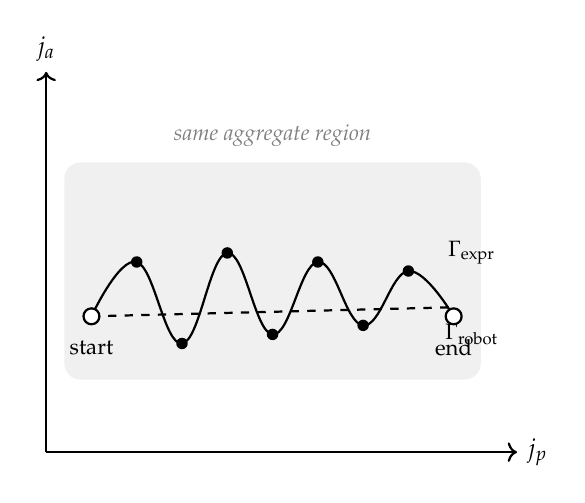
\begin{tikzpicture}[
    scale=1.15,
    axis/.style={->, thick},
    every node/.style={font=\small}
]
\draw[axis] (0,0) -- (5.2,0) node[right] {$j_p$};
\draw[axis] (0,0) -- (0,4.2) node[above] {$j_a$};

% Shaded region showing shared aggregate statistics
\fill[gray!12, rounded corners=6pt] (0.2,0.8) rectangle (4.8,3.2);
\node[font=\footnotesize\itshape, gray] at (2.5,3.5) {same aggregate region};

% Robotic trajectory — near-linear
\draw[thick, dashed]
    (0.5,1.5) -- (4.5,1.6);
\node[font=\footnotesize] at (4.7,1.3) {$\Gamma_{\mathrm{robot}}$};

% Expressive trajectory — coherent oscillation
\draw[thick]
    plot[smooth, tension=0.7] coordinates {
        (0.5,1.5)
        (1.0,2.1)
        (1.5,1.2)
        (2.0,2.2)
        (2.5,1.3)
        (3.0,2.1)
        (3.5,1.4)
        (4.0,2.0)
        (4.5,1.5)
    };
\node[font=\footnotesize] at (4.7,2.2) {$\Gamma_{\mathrm{expr}}$};

% Packet sample dots on expressive trajectory
\foreach \coord in {
    (0.5,1.5),(1.0,2.1),(1.5,1.2),(2.0,2.2),
    (2.5,1.3),(3.0,2.1),(3.5,1.4),(4.0,2.0),(4.5,1.5)
} { \fill \coord circle (1.8pt); }

% Start/end markers
\draw[fill=white, thick] (0.5,1.5) circle (2.5pt);
\draw[fill=white, thick] (4.5,1.5) circle (2.5pt);

\node[font=\footnotesize] at (0.5,1.15) {start};
\node[font=\footnotesize] at (4.5,1.15) {end};
\end{tikzpicture}
\caption{Two utterances of the same word occupy the same aggregate region of prosodic space (shaded) but differ in trajectory geometry. The robotic signal (dashed) follows a near-linear path; the expressive signal (solid) exhibits structured oscillation in the jitter dimensions, with dots indicating individual salience packet samples. Trajectory curvature and expressive coherence $\chi$ distinguish the two signals; aggregate statistics alone do not.}
\label{fig:trajectory_geometry}
\end{figure}

\begin{figure}[h]
\centering
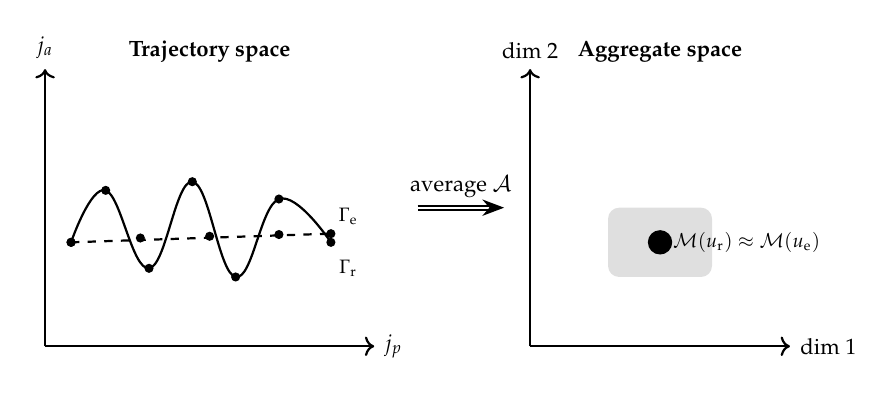
\begin{tikzpicture}[
    scale=1.1,
    every node/.style={font=\small},
    arr/.style={-{Stealth}, thick}
]
% Left panel: trajectory space
\begin{scope}[xshift=0cm]
\draw[->, thick] (0,0) -- (3.8,0) node[right, font=\footnotesize] {$j_p$};
\draw[->, thick] (0,0) -- (0,3.2) node[above, font=\footnotesize] {$j_a$};
\node[font=\footnotesize\bfseries] at (1.9,3.4) {Trajectory space};

% Robotic path
\draw[thick, dashed] (0.3,1.2) -- (3.3,1.3);
\foreach \coord in {(0.3,1.2),(1.1,1.25),(1.9,1.27),(2.7,1.29),(3.3,1.3)}
    { \fill \coord circle (1.5pt); }

% Expressive path
\draw[thick] plot[smooth, tension=0.7] coordinates
    {(0.3,1.2)(0.7,1.8)(1.2,0.9)(1.7,1.9)(2.2,0.8)(2.7,1.7)(3.3,1.2)};
\foreach \coord in {(0.3,1.2),(0.7,1.8),(1.2,0.9),(1.7,1.9),(2.2,0.8),(2.7,1.7),(3.3,1.2)}
    { \fill \coord circle (1.5pt); }

\node[font=\scriptsize] at (3.5,0.9) {$\Gamma_{\mathrm{r}}$};
\node[font=\scriptsize] at (3.5,1.5) {$\Gamma_{\mathrm{e}}$};
\end{scope}

% Arrow
\draw[arr, double] (4.3,1.6) -- node[above, font=\footnotesize]{average $\mathcal{A}$} (5.3,1.6);

% Right panel: embedding / aggregate space
\begin{scope}[xshift=5.6cm]
\draw[->, thick] (0,0) -- (3.0,0) node[right, font=\footnotesize] {dim 1};
\draw[->, thick] (0,0) -- (0,3.2) node[above, font=\footnotesize] {dim 2};
\node[font=\footnotesize\bfseries] at (1.5,3.4) {Aggregate space};

% Both collapse to same region
\fill[gray!25, rounded corners=4pt] (0.9,0.8) rectangle (2.1,1.6);
\fill (1.5,1.2) circle (4pt);
\node[font=\scriptsize] at (2.5,1.2) {$\mathcal{M}(u_{\mathrm{r}}) \approx \mathcal{M}(u_{\mathrm{e}})$};
\end{scope}
\end{tikzpicture}
\caption{Failure mode of aggregate-only analysis. In trajectory space (left), the robotic path $\Gamma_{\mathrm{r}}$ (dashed) and expressive path $\Gamma_{\mathrm{e}}$ (solid) are geometrically distinct. After averaging via $\mathcal{A}$ (right), both collapse to the same region of aggregate feature space, making them indistinguishable. Expressive coherence $\chi$ and trajectory-level DTW are required to recover the distinction.}
\label{fig:embedding_collapse}
\end{figure}


\section{Trajectory Regimes and Ergodic Writing Dynamics}

\noindent\textit{This section formalizes an observed phenomenon in human writing systems: the switching between continuous and discrete inscription modes---cursive versus print, gesture input versus letter-by-letter typing. We show that this switching is governed by trajectory predictability and corresponds to an ergodic exploration of modal space, directly instantiating the word basin architecture of Section~\ref{eq:basin}. Hyperbionic rendering makes this latent control variable explicit as a typographic invariant.}

\subsection{Two Inscription Regimes}

Human writing systems exhibit two dynamically distinct regimes of trajectory production. Cursive handwriting, swipe-based keyboard input, and fluent motor execution form the \emph{continuous regime} $\Gamma_{\mathrm{cont}}$: low segmentation, smooth curvature, high coherence, and a single motor plan executed without inter-symbol resets. Printed handwriting, letter-by-letter typing, and deliberate construction form the \emph{discrete regime} $\Gamma_{\mathrm{disc}}$: explicit segmentation, piecewise structure, and a separate motor plan per glyph.

These regimes are not stylistic choices. They are dynamical responses to the predictability of the underlying trajectory. Writers spontaneously switch from cursive to print when encountering an unfamiliar or ambiguous word, and revert to cursive once familiarity is restored. The same behaviour appears in trace-based mobile keyboards: a common word is entered as a single continuous swipe gesture (trajectory collapse onto a stored basin); an unknown or ambiguous word forces discrete letter-by-letter entry. The switching is governed by the same mechanism in both cases, and that mechanism is local uncertainty about trajectory continuation.

\subsection{Predictability and Regime Selection}

Let $H_i$ denote the local continuation entropy at token $T_i$, defined as

\begin{equation}
H_i = -\sum_j P\!\bigl(\Gamma_{i+1} = j \mid \Gamma_{\leq i}\bigr)\log P\!\bigl(\Gamma_{i+1} = j \mid \Gamma_{\leq i}\bigr).
\label{eq:Hi}
\end{equation}

The observed writing behaviour defines an implicit \emph{trajectory regime selector}:

\begin{equation}
\mathcal{R}(H_i) =
\begin{cases}
\Gamma_{\mathrm{cont}} & \text{if } H_i < \tau, \\
\Gamma_{\mathrm{disc}} & \text{if } H_i \geq \tau,
\end{cases}
\label{eq:regime}
\end{equation}

where $\tau$ is a threshold set by motor and cognitive constraints. Below threshold, continuation is sufficiently predictable that the trajectory can be executed as a single motor plan; the writer does not need to specify each symbol explicitly. Above threshold, continuation is ambiguous and the trajectory must be constructed symbol by symbol.

\begin{proposition}[Predictability--Continuity Correspondence]
Low-entropy trajectory regions admit continuous motor execution; high-entropy regions require discrete reconstruction. The transition is governed by $\mathcal{R}(H_i)$.
\end{proposition}

The formal and semantic connotations of the two regimes differ because they carry different trajectory information. Cursive encoding is used for well-integrated, frequently traversed paths and carries a signal of fluency, familiarity, and register; printed encoding is used for careful specification and carries a signal of precision, formality, or uncertainty. These are not arbitrary conventions but consequences of the underlying trajectory structure: continuous flow through a high-density basin versus discrete construction outside one.

\subsection{Word Basins and Ergodic Writing}

The regime selection connects directly to the word basin architecture of Section~\ref{eq:basin}. Let $\mathcal{B} \subset V$ denote a word basin---a high-density region of modal space corresponding to a frequently produced trajectory. Then:

\begin{equation}
\Gamma \in \mathcal{B} \;\Rightarrow\; \Gamma \approx \Gamma_{\mathrm{cont}},
\qquad
\Gamma \notin \mathcal{B} \;\Rightarrow\; \Gamma \approx \Gamma_{\mathrm{disc}}.
\label{eq:basinregime}
\end{equation}

Over extended writing, the process alternates between continuous traversal of high-density basins and discrete exploration of low-density regions. This alternation constitutes an ergodic sampling of trajectory space.

\begin{definition}[Ergodic Writing Process]
A writing process is \emph{ergodic over trajectory space} if, over time, it samples both high-density (continuous) and low-density (discrete) regions of $V$, with transitions governed by local predictability $H_i$.
\end{definition}

Ergodicity in this sense is not a metaphor: it means that the full modal space is eventually traversed by any sufficiently productive writer, with the density of traversal reflecting the frequency distribution of encountered trajectories. Frequently written words accumulate dense basins and are executed continuously; rare or technical words are constructed discretely each time, gradually building thinner basins through repetition.

\subsection{Gesture Input as Trajectory Collapse}

Swipe-based keyboards instantiate the same regime selection digitally. A gesture $\Gamma_{\mathrm{in}}$ is matched against stored word basins $\{\mathcal{W}_i\}$ via the coherence functional:

\begin{equation}
\hat{i} = \arg\max_i\, \mathcal{C}_{\mathrm{DTW}}(\Gamma_{\mathrm{in}}, \mathcal{W}_i),
\label{eq:swype}
\end{equation}

with acceptance if $\mathcal{C}_{\mathrm{DTW}} > \theta$. If no basin exceeds threshold, the system declines to resolve the gesture and prompts discrete letter entry. This is structurally identical to the regime selector \eqref{eq:regime}: ambiguity forces discretization, and the threshold $\theta$ plays the same role as $\tau$.

\begin{proposition}[Trajectory Collapse Condition]
Continuous gesture input is admissible if and only if the incoming trajectory collapses onto a unique basin under the DTW coherence functional \eqref{eq:swype}. Otherwise, discrete specification is required. The admissibility condition is the digital analogue of handwriting regime selection.
\end{proposition}

The connection to the biological coupling proposition is immediate: gesture input systems that model the trajectory rather than the symbol sequence are, by the same argument, more robust to ambiguity and more sensitive to expressive variation. A swipe keyboard that tracks jitter coherence $\chi$ in the gesture would distinguish deliberate slow tracing (high $\chi$, low $H$) from rapid ambiguous sweeping (low $\chi$, high $H$) and apply different recognition strategies accordingly.

\subsection{Hyperbionic Rendering of Trajectory Regimes}

The regime structure is a latent invariant of natural writing that conventional typography discards: plain text makes no distinction between a word entered with high fluency and one laboriously constructed. Hyperbionic rendering makes this invariant explicit by extending the parameter vector $p_i$ with a continuity parameter $c_i$ derived from predictability:

\begin{equation}
c_i = \exp(-\lambda H_i) \;\in\; (0, 1],
\label{eq:ci}
\end{equation}

where $\lambda > 0$ scales the sensitivity to entropy. The rendering operator $R$ maps $c_i$ to typographic continuity:

\begin{align}
c_i \to 1 &\;\Rightarrow\; \text{smooth, connected glyph flow (continuous regime)}, \notag\\
c_i \to 0 &\;\Rightarrow\; \text{segmented, discrete glyph rendering (discrete regime)}.
\label{eq:rendering_regime}
\end{align}

\begin{center}
\hyperstrong{Continuity is a visible invariant of predictability.}
\end{center}

This makes explicit what is implicit in handwriting: the degree to which a trajectory is known in advance becomes a visual property of the rendered text. A reader encountering a word rendered in high-continuity mode receives a signal not only about its prosodic structure but about its familiarity in the producing context---the typographic equivalent of the cursive encoding of fluency.

\begin{proposition}[Regime Invariance]
Trajectory regime (continuous versus discrete) is an invariant under admissible projection. Any representation that collapses regime distinctions discards information about predictability, ergodic position in trajectory space, and cognitive load. Plain text collapses this invariant; Hyperbionic text preserves it.
\end{proposition}

The continuity parameter $c_i$ is co-registered with the expressive coherence $\chi$: high $\chi$ with high $c_i$ indicates fluent expressive performance; high $\chi$ with low $c_i$ indicates controlled expressive production in an unfamiliar register; low $\chi$ with high $c_i$ indicates fluent but metrically regular output; low $\chi$ with low $c_i$ indicates constructed, noise-dominated signal. These four regimes correspond to distinguishable positions in the joint salience space $(\mathbf{s}, c_i)$ and admit different rendering strategies.

\begin{center}
\hyperemph{Fluency is not only speed; it is continuity of trajectory through known space.}
\end{center}

\subsection{Experimental Prediction: Keyboard Layout Transfer and Basin Depth}

The ergodic writing framework generates a falsifiable prediction that can be tested without specialised equipment. Consider a participant whose dominant layout is QWERTY. When transcribing on a non-dominant layout such as Dvorak, the familiar motor trajectories for common words are no longer available as continuous stored plans: the key positions differ, so the motor basin has different coordinates in the new layout's parameter space. The participant must reconstruct each word more explicitly.

The prediction is that this transfer cost is not uniform across words. Let $t(w, L)$ denote the time to produce word $w$ on layout $L$. A linear model gives

\begin{equation}
t(w, L) = \alpha_L \cdot n(w) + \beta_L \cdot H(w) + \varepsilon,
\label{eq:transfermodel}
\end{equation}

where $n(w)$ is word length, $H(w)$ is the continuation entropy (unfamiliarity) of the word, and $\alpha_L$, $\beta_L$ are layout-specific coefficients. The core prediction is:

\begin{equation}
\beta_{\mathrm{Dvorak}} > \beta_{\mathrm{QWERTY}},
\label{eq:transferpred}
\end{equation}

for a QWERTY-dominant participant. Unfamiliar words, which require letter-by-letter reconstruction regardless of layout, incur a disproportionately larger latency penalty under the non-dominant layout because familiar words have motor basins in QWERTY space that partially transfer (via shared ergodic structure), while unfamiliar words have no such basins in either layout and must be constructed from scratch in a space the participant does not know. The ratio $\beta_L / \alpha_L$ measures how much worse entropy is relative to length in each layout: a higher ratio under Dvorak confirms that trajectory basin depth, not raw length, is the primary determinant of non-dominant layout cost.

\begin{proposition}[Differential Transfer Prediction]
Under the ergodic writing model, the latency penalty for unfamiliar words under a non-dominant keyboard layout exceeds the penalty for familiar words by an amount proportional to the depth of the motor basin deficit: $\beta_{\mathrm{Dvorak}} - \beta_{\mathrm{QWERTY}} \propto \Delta_{\mathrm{basin}}$, where $\Delta_{\mathrm{basin}}$ measures the average difference in basin density between the two layouts for the word set.
\end{proposition}

The same prediction extends to gesture-based input. On a swipe keyboard, words for which the participant has a stable continuous gesture should transfer poorly to an unfamiliar layout (because the spatial gesture path changes), while words that were always typed discretely should transfer approximately equally. This distinguishes two populations of words in any individual's writing: those stored as continuous motor trajectories (basin residents) and those always constructed symbol by symbol (basin non-residents).


\section{Variational Reconstruction Principle}

\noindent\textit{The persistence and RSVP interpretations of the preceding sections suggest a compact variational principle that unifies the entire pipeline. The RSVP field does not merely evolve by local update rules; it evolves toward configurations that maximize stable reconstructibility across admissible projections. This section states that principle precisely and shows that Hyperbionic rendering is its typographic instantiation.}

Let $X(t) = (\Phi(t), \mathbf{v}(t), S(t))$ denote the RSVP field state, and let $\{\mathcal{P}_k\}_{k=1}^K$ be a family of projection operators into observable media: acoustic signal, modal memory, typographic rendering, motor gesture, and contextual markup. A configuration is admissible when its projections remain mutually reconstructible.

Define the reconstruction loss

\begin{equation}
\mathcal{R}[X]
= \sum_{k,\ell} \int_0^T
d_k\!\left(\mathcal{P}_k(X(t)),\; \mathcal{T}_{k\ell}\,\mathcal{P}_\ell(X(t))\right)^2 dt,
\label{eq:RecLoss}
\end{equation}

where $d_k$ is the metric in the $k$-th observation space and $\mathcal{T}_{k\ell}$ is the translation operator from modality $\ell$ to modality $k$. This term penalises disagreement between different renderings of the same underlying field. The total action is

\begin{equation}
\mathcal{A}[X]
= \int_0^T \mathcal{L}_{\mathrm{RSVP}}(X, \partial_t X)\, dt
\;+\; \lambda\, \mathcal{R}[X]
\;+\; \mu \int_0^T S(t)^2\, dt.
\label{eq:TotalAction}
\end{equation}

The first term enforces the native RSVP dynamics. The second enforces cross-modal reconstructibility. The third penalises entropy accumulation, preventing the system from preserving structure only by allowing indefinite uncertainty growth. The variational principle is

\begin{equation}
X^* = \arg\min_X \mathcal{A}[X].
\label{eq:VarPrinciple}
\end{equation}

\begin{definition}[Reconstructive Meaning]
\label{def:reconmeaning}
A structure $Y$ has reconstructive meaning relative to a projection family $\{\mathcal{P}_k\}$ if there exists an admissible RSVP field configuration $X^*$ such that $Y = \mathcal{P}_k(X^*)$ for some $k$, and $X^*$ minimizes the reconstruction action $\mathcal{A}[X]$.
\end{definition}

This definition separates meaning from mere signal presence. A signal fragment may exist in one modality without being meaningful if it cannot be reconciled with the others. Conversely, a weak or partial cue may carry high meaning if it reliably reconstructs the same invariant across modalities --- precisely the ecphory structure of Section~9.

\begin{proposition}[Meaning as Projection-Stable Reconstruction]
If $X^*$ minimizes $\mathcal{A}[X]$, then any two admissible projections $\mathcal{P}_k(X^*)$ and $\mathcal{P}_\ell(X^*)$ are equivalent up to bounded reconstruction error. Meaning is preserved not by identity of medium but by stability of reconstruction across media.
\end{proposition}

Hyperbionic text is one projection in this variational system. Its role is not to decorate lexical tokens but to reduce $\mathcal{R}[X]$: it makes the typographic projection more faithful to the acoustic, motor, and contextual projections of the same underlying field. Plain text has high reconstruction loss because it collapses prosody, cadence, gesture, and environmental grounding. Hyperbionic text lowers that loss by restoring enough visual structure for the reader to reconstruct the field trajectory.

The Hyperbionic rendering operator $R$ is therefore a reconstruction-energy minimizer: it chooses visual transformations that preserve prosodic invariants while satisfying legibility constraints. The optimal rendering is not the most expressive rendering, but the one that minimizes reconstruction loss subject to perceptual admissibility:

\begin{equation}
R^* = \arg\min_R \left(\mathcal{R}[R] + \nu\, C[R]\right),
\label{eq:OptR}
\end{equation}

where $C[R]$ is the typographic constraint energy. This closes the loop between RSVP dynamics and Hyperbionic typography: both are governed by the same principle of constraint-preserving reconstruction under the variational action $\mathcal{A}$.


\section{Spherepop Integration: Prosody as Irreversible Constraint Accumulation}

\noindent\textit{This section situates the Hyperbionic pipeline within the Spherepop process-oriented architecture. Spherepop models computation as irreversible event history: each event is a committed, non-retractable pop that accumulates constraint. Prosodic trajectories, TARTAN tiles, and the differential prosodic envelope all have precise Spherepop interpretations that deepen the invariant-preservation account without introducing new machinery.}

\subsection{Trajectories as Event-Historical Traces}

In Spherepop, the fundamental computational object is not a state but a history: a sequence of pops, each of which commits a constraint that cannot be undone by future events. The trajectory $\Gamma = \{Z_\alpha(t_k)\}_{k=1}^N$ has exactly this structure. Each salience packet $\mathcal{P}_k$ is an event: a peak detection that is irreversible (the peak either occurred or it did not), that commits a constraint (the inter-peak interval $\Delta t_k$ and amplitude $a_k$ are recorded as fixed values), and that is non-retractable (later packets cannot alter earlier ones, only extend the history).

The trajectory $\Gamma$ is therefore not a sequence of states but a \emph{constraint history}: a record of irreversible commitments made by the acoustic signal as it evolved. This matches the Spherepop semantics precisely. The modal coordinate $Z_\alpha(t_k) = Q(\phi(\mathcal{P}_k))$ is the Spherepop output of the $k$-th pop: a committed, quantized encoding of the constraints imposed by that event. Aggregation $\mathcal{M}(u) = \mathcal{A}(\{P_k\})$ is a summary functional over the history, not the history itself — the distinction the paper drew between packets as fundamental and the prosodic vector as derived.

\begin{definition}[Prosodic Event History]
\label{def:eventhistory}
The prosodic event history of a waveform $u(t)$ is the ordered sequence
\begin{equation}
\mathcal{H}(u) = \bigl(\mathcal{P}_1, \mathcal{P}_2, \ldots, \mathcal{P}_N\bigr),
\label{eq:eventhistory}
\end{equation}
where each $\mathcal{P}_k$ is a committed, irreversible constraint on the prosodic trajectory, and the trajectory $\Gamma$ is the pushforward of $\mathcal{H}(u)$ under the quantization map $Q \circ \phi$.
\end{definition}

\subsection{TARTAN Tiles as Recursive Constraint Buffers}

In Spherepop, complex computations are structured by layered pops: outer pops accumulate constraints over longer histories; inner pops record local events. The TARTAN hierarchy $\{\mathcal{T}_\ell(\Gamma)\}_{\ell=0}^L$ is exactly this structure.

Each tile $\tau_{\ell,j} = (\bar{Z}_{\ell,j}, \Sigma_{\ell,j}, \eta_{\ell,j}, \chi_{\ell,j}, b_{\ell,j})$ is a committed summary of the constraint history within its temporal extent. The boundary flag $b_{\ell,j}$ is a Fracture record: a committed observation that a silence or voiced-segment boundary occurred within the tile, which cannot be revised by finer-grained tiles at level $\ell+1$ or coarser tiles at level $\ell-1$. The propagation of $b_{\ell,j}$ up the hierarchy is therefore not interpolation or estimation — it is constraint inheritance: coarser tiles inherit the irreversibility commitments of the finer tiles they summarize.

\begin{proposition}[Fracture as Irreversible Commitment]
A Fracture marker $b_{\ell,j} = 1$ at level $\ell$ is an irreversible commitment: it forecloses any reconstruction that would require aligning voiced content across the silence boundary recorded in tile $(\ell, j)$. This commitment is inherited by all coarser tiles that contain $(\ell, j)$, and cannot be revised by evidence from finer tiles.
\end{proposition}

This is the Spherepop semantics of TARTAN: each tile pop commits a constraint on which alignments are admissible, and the DTW coherence functional \eqref{eq:dtwG} respects those commitments by restricting alignment paths to within connected voiced components $\Gamma_m$ of the decomposition \eqref{eq:decomp}.

\subsection{Differential Envelopes as Irreversibility Encoding}

The differential prosodic envelope $\nabla p_i = p_i - p_{i-1}$ introduced in Section~20 encodes the rate of change between adjacent tokens. Its Spherepop interpretation is precise: it records the irreversibility of the transition between consecutive events.

A pitch drop from $f_{i-1}$ to $f_i$ is not equivalent to a pitch rise of the same magnitude in the opposite direction, even if the endpoint $f_i$ is the same. The prosodic meaning of a descent is not the time-reversal of an ascent: falling intonation encodes finality or assertion in many languages; rising intonation encodes continuation or query. The signed gradient $\nabla f_i < 0$ versus $\nabla f_i > 0$ encodes a directional commitment that is irreversible in the Spherepop sense — the history of how a pitch value was reached is semantically distinct from the value itself.

Formally, the extended parameter vector $\tilde{p}_i = (p_i, \nabla p_i)$ is an event in the event history $\mathcal{H}(u)$: it commits not only the current parameter value but the direction of arrival, which cannot be erased by subsequent values. This is why the salience-weighted rendering operator $R_s$ in Section~20 should in principle also weight the differential components: a large signed gradient with high salience (a sharp, salient pitch drop) should render as a visually committed directional transition, not merely as a difference in endpoint values.

\subsection{Reading as Constraint Accumulation}

The Spherepop model of computation as constraint accumulation gives a precise account of what a reader does when encountering Hyperbionic text. Reading is not a process of decoding stored symbols. It is a process of accumulating the constraint history of the speaker's vocal intent, pop by pop, as the eye traverses the rendered trajectory.

Each Hyperbionic token $\mathcal{H}(T_i, p_i)$ is a pop in the reader's accumulation process: it commits a constraint on the prosodic trajectory that the reader is reconstructing. High-salience tokens ($s_i \approx 1$) commit strong constraints; low-salience tokens ($s_i \approx 0$) commit weak constraints that leave the trajectory under-determined at that point. The accumulated history of these commitments is the reader's internal representation of the speaker's prosodic trajectory — not a symbol sequence, not a feature vector, but a Spherepop constraint history that can be used to re-enact the original acoustic event history $\mathcal{H}(u)$ within the bounds allowed by the reconstruction loss $\mathcal{R}[R]$.

\begin{center}
\hyperemph{A Hyperbionic document is a Spherepop program for reconstructing a voice.}
\end{center}

The irreversibility of this process is what gives it semantic force. A reader who has accumulated the constraint history of a falling-intonation declarative cannot simply re-read it as a rising-intonation query by reversing the differential envelope: the boundary constraints, salience weights, and coherence values committed at each pop foreclose that reinterpretation. The trajectory is directed; reading it accumulates irreversible commitments that constrain interpretation in exactly the way the speaker's acoustic event history constrained the original prosodic trajectory.


\section{Triangular Equivalence}

The full equivalence \eqref{eq:fullequiv} has a natural geometric form. The three trajectory representations---audio, memory, and text---are not linearly ordered but mutually projectable: any two can be converted to the third via the operators defined in the preceding sections. This mutual projectability is represented in Figure~\ref{fig:triangle}.

\begin{figure}[h]
\centering
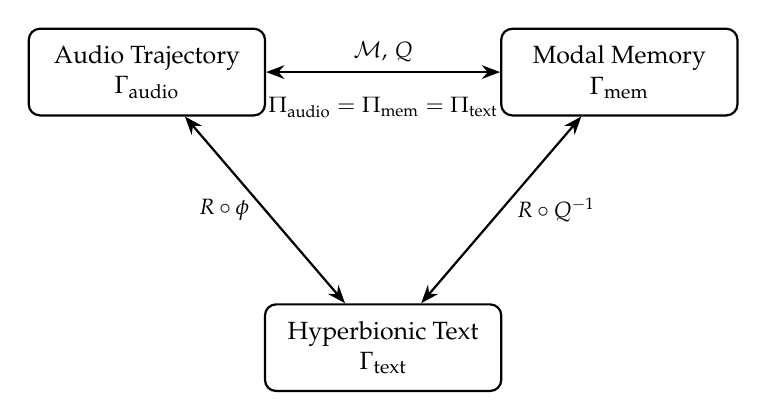
\begin{tikzpicture}[
    every node/.style={font=\small},
    box/.style={rectangle, draw, thick, rounded corners, align=center,
                minimum width=3.0cm, minimum height=1.1cm, fill=white},
    arr/.style={{Stealth}-{Stealth}, thick},
    label/.style={font=\footnotesize\itshape}
]
\node[box] (audio) at (0, 0)    {Audio Trajectory\\$\Gamma_{\mathrm{audio}}$};
\node[box] (mem)   at (6, 0)    {Modal Memory\\$\Gamma_{\mathrm{mem}}$};
\node[box] (text)  at (3, -3.5) {Hyperbionic Text\\$\Gamma_{\mathrm{text}}$};

\draw[arr] (audio) -- node[label, above]{$\mathcal{M},\,Q$} (mem);
\draw[arr] (audio) -- node[label, left, xshift=-2pt]{$R \circ \phi$} (text);
\draw[arr] (mem)   -- node[label, right, xshift=2pt]{$R \circ Q^{-1}$} (text);

\node[font=\footnotesize, align=center] at (3,-0.45)
    {$\Pi_{\mathrm{audio}} = \Pi_{\mathrm{mem}} = \Pi_{\mathrm{text}}$};
\end{tikzpicture}
\caption{Triangular equivalence of the three trajectory representations. Each vertex is a representation of the same prosodic invariant structure in a different medium. The double-headed arrows indicate structure-preserving projections in both directions. The central identity states that all three projection operators extract the same invariants from their respective media.}
\label{fig:triangle}
\end{figure}

\begin{definition}[Prosodic Invariant Field]
The \emph{prosodic invariant field} is the equivalence class of all representations---audio, modal, typographic---that preserve the projection operator $\Pi$. Formally, it is the fiber over $\Pi$ in the bundle of signal representations over the shared parameter space.
\end{definition}

The three vertices of the triangle are sections of this field over different media. The equivalence \eqref{eq:fullequiv} holds conditionally: $\Pi_{\mathrm{audio}}(u) = \Pi_{\mathrm{mem}}(Z) = \Pi_{\mathrm{text}}(R(g,p))$ if and only if the operators $R$ and $Q$ are \emph{admissible} in the sense of being invariant-preserving (no distinctions present in the parameter space are collapsed) and non-collapsing (no distinctions absent from the parameter space are introduced). This makes triangular equivalence a design criterion testable by inspection of the rendering and quantization maps.

The three sides of the triangle correspond to three distinct operations. The top edge is the Marine--MEM$|$8 chain: acoustic measurement $\mathcal{M}$ followed by fixed-point quantization $Q$, converting audio trajectories into modal lattice coordinates. The left edge is the rendering chain: the projection $\phi$ from packet space to prosodic parameter space followed by the Hyperbionic rendering operator $R$, converting audio trajectories directly into visual typography. The right edge is the reconstruction chain $R \circ Q^{-1}$: reading a Hyperbionic rendering back through the inverse quantization to recover a prosodic vector, and then synthesizing an audio trajectory consistent with that vector.

The central identity $\Pi_{\mathrm{audio}} = \Pi_{\mathrm{mem}} = \Pi_{\mathrm{text}}$ is the claim that all three projection operators extract the same invariant structure. This is not a tautology: it is a constraint on the design of the rendering operator $R$ and the quantization operator $Q$, requiring that neither introduces distinctions not present in the prosodic parameter space and neither collapses distinctions that the other preserves. A rendering operator that maps two distinct prosodic vectors to the same visual output violates the constraint; so does a quantization scheme that conflates vectors that the rendering operator distinguishes. The triangular equivalence is therefore a testable design criterion, not merely a philosophical claim.

\subsection{Categorical Structure: Functorial Projections Between Trajectory Categories}

The operators $\mathcal{M}$, $Q$, $R$, and $\mathcal{P}_{\mathrm{mim}}$ are not merely functions between representation spaces. They are structure-preserving maps between categories of trajectories, and their compositions commute up to invariant equivalence.

Define the base category $\mathbf{Traj}$ whose objects are prosodic trajectories $\Gamma \subset V = (\mathbb{R}^8, G)$ and whose morphisms are admissible transformations preserving the invariant $\mathcal{I}$. Each modality defines a subcategory:

\begin{equation}
\mathbf{Audio},\quad \mathbf{Mem},\quad \mathbf{Text},\quad \mathbf{Motor},
\label{eq:categories}
\end{equation}

where $\mathbf{Audio}$ contains waveform-parameterized trajectories, $\mathbf{Mem}$ contains modal lattice trajectories, $\mathbf{Text}$ contains Hyperbionic typographic trajectories, and $\mathbf{Motor}$ contains mimetic gesture trajectories. The operators become functors:

\begin{equation}
\mathcal{M} : \mathbf{Audio} \to \mathbf{Traj},\qquad
R : \mathbf{Traj} \to \mathbf{Text},\qquad
\mathcal{P}_{\mathrm{mim}} : \mathbf{Traj} \to \mathbf{Motor}.
\label{eq:functors}
\end{equation}

The commutativity condition --- that all paths between modalities yield the same invariant --- is expressed as a commuting diagram over four modalities:

\begin{equation}
R \circ \mathcal{M} \;\simeq\; \mathcal{P}_{\mathrm{mim}} \circ \mathcal{M},
\label{eq:commute}
\end{equation}

and analogously for all other compositions. In plain terms: whether the signal is routed audio $\to$ text, or audio $\to$ motor $\to$ text, the invariant $\mathcal{I}$ is preserved. No modality is primary; all are coordinate charts on the same underlying object.

\begin{proposition}[Functorial Characterisation of Invariant Preservation]
All modalities are functorial projections of $\mathbf{Traj}$. A representation is admissible if and only if the corresponding functor is faithful with respect to $\mathcal{I}$: it preserves morphisms that are distinct under the invariant.
\end{proposition}

The aggregation impossibility result (Section~\ref{eq:lossy_invariant}) now has a precise categorical statement: the aggregation map $\mathcal{A} : \mathbf{Traj} \to \mathbb{R}^n$ is not faithful. It collapses morphisms that are distinct in $\mathbf{Traj}$---it identifies trajectories that are geometrically different---and therefore destroys the categorical structure that carries expressive meaning. Standard acoustic embedding systems are instances of non-faithful functors; the trajectory-based architecture is an instance of a faithful one.


\section{Multimodal Disambiguation: Contextual Grounding of Prosodic Invariants}

\noindent\textit{This section addresses a structural limitation of single-modality prosodic analysis: the same invariant vector can arise from physically distinct causes. Additional modalities resolve this degeneracy not by adding information arbitrarily, but by intersecting independent constraint sets over the interpretation space.}

The prosodic measurement operator $\mathcal{M}$ is many-to-one with respect to underlying causes. The same invariant vector $\mathcal{I}(u)$ can arise from physically distinct situations: elevated energy and increased jitter might correspond to anger, physical exertion, environmental noise compensation, or distance from the microphone. Formally, there exist distinct signal contexts $x_1 \neq x_2$ such that

\begin{equation}
\mathcal{M}(u_{x_1}) = \mathcal{M}(u_{x_2}),
\label{eq:degeneracy}
\end{equation}

where $u_{x_i}$ denotes the acoustic waveform produced in context $x_i$. This degeneracy is not a failure of the measurement operator: it reflects the genuine fact that prosody is a projection of a higher-dimensional causal space onto a lower-dimensional invariant space. The invariant is real; the ambiguity lies in the inverse problem of recovering cause from invariant.

\subsection{Contextual Operators and Constraint Intersection}

The resolution is not to add more prosodic dimensions but to introduce a complementary \emph{contextual operator} $C$ that maps environmental observations into a parameter space over causes:

\begin{equation}
C : \text{environment} \to \mathbb{R}^m,
\label{eq:context}
\end{equation}

where the environment includes visual scene, spatial configuration, device state, and any other modality that constrains the causal interpretation. The joint invariant is then

\begin{equation}
\mathcal{I}_{\mathrm{joint}} = \bigl(\mathcal{I}(u),\; C(\text{environment})\bigr),
\label{eq:joint}
\end{equation}

and disambiguation is the process of finding the intersection of the prosodic and contextual constraint sets. The same prosodic vector $\mathcal{I}(u)$ combined with different contextual vectors $C$ yields different realised interpretations: elevated energy combined with visual evidence of a distant interlocutor implies distance compensation; combined with a tense facial expression at close range, it implies anger; combined with a construction-site acoustic signature, it implies environmental override.

A photograph, markup tag, or spatial sensor is not adding a new kind of information to the system; it is providing a constraint that carves the interpretation manifold $\mathcal{I}^{-1}(\mathcal{I}(u))$---the set of all contexts that produce the observed invariant---into a smaller admissible region. The disambiguation is the intersection of the prosodic fiber with the contextual constraint set.

\subsection{The Admissibility Condition on Additional Modalities}

The key design principle is not that more channels are always better. Additional modalities must be co-registered with the invariant structure: they must be aligned in time, parameterized in a space that has a well-defined projection onto the causal interpretation manifold, and consistent with the admissibility constraints already imposed on the primary prosodic channel.

Misaligned markup---irrelevant images, noisy metadata, or temporally inconsistent annotations---does not reduce ambiguity; it increases entropy in the interpretation space. In the framework of this paper, this is the multimodal analogue of spectral fracturing: additional channels that impose a reconstruction burden without contributing constraint resolution degrade the system's coherence rather than improving it. The admissibility condition on additional modalities mirrors the admissibility condition on typographic rendering: the new channel must be invariant-preserving and non-collapsing with respect to the joint interpretation space.

\subsection{Prosodic and Contextual Invariants}

The extended framework separates two roles that single-modality analysis conflates:

\begin{equation}
\underbrace{\mathcal{I}(u)}_{\text{internal dynamics}} \;\oplus\; \underbrace{C(\text{environment})}_{\text{external grounding}}.
\label{eq:separation}
\end{equation}

Prosodic invariants determine the space of possible interpretations by specifying location, curvature, and coherence in the modal parameter space. Contextual invariants determine which interpretation is realised by grounding those dynamics in external causes. One gives you the geometry of the signal; the other gives you its referent.

Hyperbionic text encodes the first term of \eqref{eq:separation}: it preserves the internal dynamics of the signal across modalities. Environmental markup---photographs, spatial tags, device-state annotations---encodes the second term. A fully grounded Hyperbionic document would carry both, making the interpretation space closed: the reader can recover not only the prosodic structure of the utterance but the causal context in which it was produced.


\section{Embodied Prosody: Mimetic Proxy, ASL Classifier Dynamics, and the Motion Layer of Meaning}

\noindent\textit{This section extends the invariant framework into embodied cognition. Prosodic trajectories are not merely acoustic features but motor-reconstructible structures whose loss under transcription produces systematic semantic impoverishment. The analysis draws a formal equivalence between speech prosody, mimetic simulation as theorized by Cox, and classifier dynamics in American Sign Language, establishing that Hyperbionic rendering restores an objectively real layer of meaning---not a stylistic enhancement.}

\subsection{Mimetic Proxy and the Motor Basis of Prosodic Meaning}

Arnie Cox's theory of music cognition proposes that perceived sound is internally reconstructed as bodily motion~\cite{Cox2016}. Listeners do not merely hear a rhythmic phrase or a melodic contour: they covertly simulate the gestures that would produce or accompany it. A staccato burst evokes short, repeated motor impulses---tapping, bouncing; a sustained legato line evokes continuous smooth extension---gliding, stretching. This \emph{mimetic proxy} relationship means that acoustic signals are interpreted through an implicit motor mapping that is prior to, and partly constitutive of, semantic content.

Spoken language carries the same structure. Clipped speech maps to discrete motor pulses; elongated vowels map to continuous extension; rising pitch maps to upward gesture; jitter and vibrato map to oscillatory motion. Two utterances can be lexically identical but mimetically distinct, inducing divergent interpretations through the motion layer rather than the symbolic layer. A repeated, bouncing rhythmic pattern in speech can signal insistence, playfulness, or agitation; words alone do not disambiguate this. The trajectory of the signal does.

Within the present framework, this mapping is not external to the signal but inherent in its trajectory representation. Let $\Gamma = \{Z_\alpha(t_k)\}$ be a prosodic trajectory in modal space $V = (\mathbb{R}^8, G)$. We define the \emph{mimetic projection operator}
\begin{equation}
\mathcal{P}_{\mathrm{mim}} : \Gamma \;\longrightarrow\; \mathcal{G},
\label{eq:mimetic}
\end{equation}
where $\mathcal{G}$ is a space of motor gestures parameterized by direction, amplitude, periodicity, and continuity. The operator $\mathcal{P}_{\mathrm{mim}}$ maps prosodic curvature and coherence into reconstructible motion primitives.

\begin{proposition}[Mimetic Equivalence]
For any prosodic trajectory $\Gamma$, there exists a motor trajectory $\mathcal{P}_{\mathrm{mim}}(\Gamma) \in \mathcal{G}$ such that perception of $\Gamma$ is mediated by covert reconstruction of $\mathcal{P}_{\mathrm{mim}}(\Gamma)$, up to equivalence in curvature and coherence. Representations that collapse curvature and coherence eliminate the mimetic proxy and thereby impoverish meaning.
\end{proposition}

\subsection{Transcription as Destruction of the Mimetic Layer}

Standard transcription collapses the trajectory $\Gamma$ to a sequence of lexical tokens $\{T_i\}$, eliminating curvature and coherence:
\begin{equation}
\Gamma \;\longrightarrow\; \{T_i\},
\label{eq:collapse}
\end{equation}
with no invertible mapping. The mimetic projection $\mathcal{P}_{\mathrm{mim}}$ is therefore undefined on plain text, forcing the reader to reconstruct motion from prior experience:
\begin{equation}
\{T_i\} \;\to\; \text{inferred } \Gamma \;\to\; \mathcal{P}_{\mathrm{mim}}(\Gamma).
\label{eq:inference}
\end{equation}
This is the proximate source of prosodic semantic ambiguity: distinct trajectories $\Gamma_1 \neq \Gamma_2$ collapse to the same token sequence yet induce different mimetic reconstructions. The ambiguity is not resolved by lexical content but by the motion layer that transcription destroyed. A reader with a rich internal trajectory space from extensive listening can partially reconstruct the motion; a reader without that space cannot. In both cases, the text forces inference where encoding is possible.

\subsection{ASL Classifier Dynamics as Proof of Existence}

American Sign Language provides a system in which motion parameters are explicitly semantic, establishing beyond dispute that the motion layer of meaning can be systematically encoded and perceived~\cite{Liddell2003,Emmorey2002}. Classifier constructions in ASL encode semantic aspect directly through motion properties: repetition of a movement encodes iterative or ongoing action (the signed analogue of a gerund or progressive aspect); increased velocity encodes urgency or intensity; expanded spatial extent encodes scale or magnitude; path shape encodes spatial semantics; oscillatory motion encodes instability or continuity.

The structural parallel to the present framework is precise. ASL classifier semantics can be expressed as:
\begin{equation}
\text{meaning}_{\mathrm{ASL}} = (\text{handshape},\; \text{motion trajectory}),
\label{eq:asl}
\end{equation}
which is formally isomorphic to the semantic decomposition of Definition~\ref{def:semantic} in the prosodic domain:
\begin{equation}
\text{meaning}_{\mathrm{prosodic}} = (\text{location},\; \text{curvature},\; \text{coherence}).
\label{eq:prosodic_meaning}
\end{equation}
In both systems, the motion component is not decorative but constitutive: removing it changes the meaning, not merely the style. ASL does not lose this layer because it encodes it explicitly in a spatial-gestural medium. Spoken language contains the same layer; written language discards it.

We formalize the ASL-to-prosody correspondence as a \emph{classifier transformation} acting on trajectories:
\begin{equation}
\Gamma \;\mapsto\; \Gamma' = \mathcal{C}_{\mathrm{cls}}(\Gamma),
\label{eq:classifier}
\end{equation}
where $\mathcal{C}_{\mathrm{cls}}$ applies structured modifications such as temporal tiling (repetition $\leftrightarrow$ iterative aspect), amplitude scaling (magnitude $\leftrightarrow$ intensity), and time compression (acceleration $\leftrightarrow$ urgency). Each of these transformations modifies the curvature and temporal density of $\Gamma$ in a principled way, corresponding to the motion modifications of ASL classifier constructions.

\begin{proposition}[Aspect Encoding via Trajectory Transformation]
Semantic aspect---iterative, continuous, urgent, attenuated---is representable as a transformation on prosodic trajectory curvature and temporal density. Two utterances with identical lexical content but distinct $\mathcal{C}_{\mathrm{cls}}$ transformations are semantically non-equivalent. Plain text collapses this distinction; Hyperbionic text preserves it.
\end{proposition}

\subsection{Hyperbionic Rendering as Mimetic Restoration}

Hyperbionic text restores the mimetic layer by rendering trajectory parameters directly into visual degrees of freedom. The rendering operator $R$ maps the prosodic trajectory to a typographic trajectory:
\begin{equation}
\Gamma \;\xrightarrow{\;R\;}\; \Gamma_{\mathrm{text}} = \{p_i\},
\label{eq:rendertraj}
\end{equation}
where $p_i$ encodes local energy, duration, jitter, and coherence for the $i$-th token. The mimetic projection is then preserved across the rendering:
\begin{equation}
\mathcal{P}_{\mathrm{mim}}(\Gamma) \;\equiv\; \mathcal{P}_{\mathrm{mim}}(\Gamma_{\mathrm{text}}).
\label{eq:mimequiv}
\end{equation}

The classifier correspondence is concrete. A bouncing or iterative prosodic pattern---high-$\chi$ oscillatory jitter at short periodicity---appears in Hyperbionic rendering as repeated typographic modulation: micro-variations in weight, spacing, or baseline that recur with the same period as the prosodic oscillation. This is the typographic gerund: iterative motion encoded as structured repetition in the visual field. A sustained, continuous prosodic pattern---low jitter, long duration, smooth energy envelope---appears as continuous spatial deformation: gradually increasing size or baseline displacement across the token sequence. A compressed, urgent pattern---high peak density, rapid energy rise---appears as condensed spacing with elevated weight. Each of these corresponds exactly to a classifier transformation $\mathcal{C}_{\mathrm{cls}}$ in the ASL sense.

\begin{center}
\hyperstrong{Hyperbionic text is a perceptible motion field.}
\end{center}

\begin{definition}[Embodied Semantic Field]
The embodied semantic field of an utterance is the pair
\begin{equation}
\mathcal{E}(\Gamma) = \bigl(\Gamma,\; \mathcal{P}_{\mathrm{mim}}(\Gamma)\bigr),
\label{eq:embodied}
\end{equation}
combining trajectory geometry with its motor reconstruction. A representation is semantically complete if and only if it preserves $\mathcal{E}$.
\end{definition}

Plain text preserves lexical identity and discards $\mathcal{E}$. Hyperbionic text preserves $\mathcal{E}$ by encoding $\Gamma$ in a perceptible visual form from which $\mathcal{P}_{\mathrm{mim}}$ can be reconstructed. It is therefore not an augmentation of text but a recovery of the embodied semantic field that phonological transcription structurally eliminates.

\subsection{Semantic Disambiguation via Trajectory Visibility}

The restoration of trajectory structure resolves the degeneracy identified in Section~\ref{eq:degeneracy}. Let $\Gamma_1 \neq \Gamma_2$ be two trajectories with identical lexical projections:
\begin{equation}
\{T_i\}(\Gamma_1) = \{T_i\}(\Gamma_2), \qquad \Gamma_{\mathrm{text}}(\Gamma_1) \neq \Gamma_{\mathrm{text}}(\Gamma_2).
\label{eq:disambig}
\end{equation}
The Hyperbionic representation preserves distinctions that plain text collapses, allowing direct perception of differences in cadence, emphasis, and mimetic character. A transcription that records not only what a speaker said but how their voice moved encodes accent, emotional register, and communicative intent as geometric properties of the rendered text rather than as metadata or stylistic annotation.

\begin{center}
\hyperemph{Meaning is not only what is said, but how it moves.}
\end{center}


\section{Persistence, Interference, and Reconstruction}

\noindent\textit{This section reinterprets the pipeline operators as a selection process rather than an extraction process. Structure is not found in signals; it is stabilized across repeated projections. Components that remain coherent under multiple transforms contribute to the invariant; those that cannot be jointly reconstructed from multiple views do not. This reframing replaces the implicit notion of feature extraction with a dynamical criterion of interference-stable persistence.}

\subsection{Structure as Interference-Stable Content}

The pipeline

\begin{equation}
u(t) \;\longrightarrow\; \{\mathcal{P}_k\} \;\longrightarrow\; \Gamma
\label{eq:pipeline_again}
\end{equation}

is conventionally read as feature extraction: each operator reveals a latent property of the signal. This reading is incomplete. It assumes that structure is localized and static, waiting to be uncovered. In practice, meaningful structure is not given at a point; it is stabilized across transformations.

Let $\{\mathcal{P}_k\}$ be a family of projections acting on a trajectory $\Gamma$. Each projection produces a partial observation, but no single projection is authoritative. Structure emerges through agreement across projections: components that are compatible across multiple $\mathcal{P}_k$ reinforce and persist; components that are incompatible destructively cancel. We therefore reinterpret the invariant $\mathcal{I}(\Gamma)$ not as a set of extracted features but as a configuration satisfying a consistency condition:

\begin{equation}
\mathcal{I}(\Gamma) \;\sim\; \bigcap_k \mathrm{Stab}(\mathcal{P}_k(\Gamma)),
\label{eq:stab}
\end{equation}

where $\mathrm{Stab}(\mathcal{P}_k(\Gamma))$ is the set of trajectory configurations stable under projection $\mathcal{P}_k$. Structure is what survives interference. This replaces "feature extraction" with a selection principle: only those aspects of $\Gamma$ that remain coherent across multiple transforms contribute to $\mathcal{I}$.

This perspective retroactively clarifies the salience formula $s = 1/(1 + \overline{j_p} + \overline{j_a})$: salience is not a measure of amplitude but of cross-projection stability. A peak with high amplitude but inconsistent timing across analysis windows contributes less to $\mathcal{I}$ than a quieter peak whose temporal position is stable across the EMA projection, the period validity gate, and the harmonic coherence estimate. Salience is persistence, not energy.

\subsection{Admissibility as Graded Persistence}

Admissibility has previously been defined as a binary constraint: a trajectory satisfies $C[\gamma] \leq C_{\max}$ or it does not. This can be refined into a graded dynamical property.

Consider a composition chain of operators acting on $\Gamma$:

\begin{equation}
\Gamma
\;\xrightarrow{\mathcal{P}_{k_1}}\;
\mathcal{P}_{k_1}(\Gamma)
\;\xrightarrow{\mathcal{P}_{k_2}}\;
\cdots
\;\xrightarrow{\mathcal{P}_{k_n}}\;
\mathcal{P}_{k_n} \circ \cdots \circ \mathcal{P}_{k_1}(\Gamma).
\label{eq:chain}
\end{equation}

A component of $\Gamma$ is \emph{persistent} if it remains reconstructible under such compositions. Define the persistence functional:

\begin{equation}
\Pi(\Gamma) = \int_0^T \mathbf{1}\bigl[\text{reconstructible at depth } t\bigr]\, dt,
\label{eq:Pifunc}
\end{equation}

measuring the total duration over which $\Gamma$'s structure survives the operator chain. Admissibility then becomes graded: highly persistent components dominate the representation; transient components naturally attenuate without requiring explicit removal. What appears as filtering is the failure of unstable components to propagate through the chain. The constraint energy $C[\gamma]$ is a proxy for low persistence: high misalignment $\theta$, high uncertainty $S$, and high vorticity $\xi$ all correspond to components that do not survive repeated projection.

\subsection{Reconstruction as the Criterion of Meaning}

Let $\{\mathcal{P}_k(\Gamma)\}$ be the set of projections of a trajectory. A candidate representation $\hat{\Gamma}$ is consistent if it reproduces these projections within tolerance:

\begin{equation}
\mathcal{P}_k(\hat{\Gamma}) \approx \mathcal{P}_k(\Gamma) \quad \forall k.
\label{eq:consistency}
\end{equation}

Define the coherence supremum:

\begin{equation}
\mathcal{I}(\Gamma) = \sup_{\hat{\Gamma}}\; \mathrm{Cons}\!\bigl(\hat{\Gamma},\, \{\mathcal{P}_k(\Gamma)\}\bigr),
\label{eq:coherence_sup}
\end{equation}

where $\mathrm{Cons}$ measures the degree to which $\hat{\Gamma}$ satisfies \eqref{eq:consistency}. Meaning is identified not with what is stored but with what can be reconstructed: a structure is meaningful to the extent that it admits a stable inverse across the projection family. Components that cannot be jointly reconstructed from multiple views do not contribute to $\mathcal{I}$, and therefore do not participate in the invariant.

This reframing resolves a conceptual ambiguity that the preceding sections leave implicit. Hyperbionic text does not contain the prosodic signal in the way that a recording contains audio. It is a projection of $\Gamma$ into typographic parameter space, and a reader does not decode that projection but reconstructs $\Gamma$ from it using their stored trajectory space. What the Hyperbionic rendering does is shift the reconstruction burden from inference (guessing the trajectory from lexical cues alone) to perception (reading the trajectory from explicit visual parameters). The reconstruction still occurs; what changes is how much of the work is done by the rendering versus the reader's internal models.

\subsection{Persistent Substrate and Rendered Observation}

The distinction between persistent and transient components induces a natural architectural separation. Write

\begin{equation}
u(t) = X(t) + \varepsilon(t),
\label{eq:substrate_noise}
\end{equation}

where $X(t)$ is the persistent substrate and $\varepsilon(t)$ is transient noise. The projections $\{\mathcal{P}_k\}$ act primarily as observation operators, producing rendered views of $X(t)$ modulated by $\varepsilon(t)$. The role of the pipeline is not to store rendered outputs but to recover $X(t)$ as the invariant structure that generates them.

In this sense, text, symbols, and all discrete outputs are not fundamental objects. They are downstream renderings of a continuously evolving substrate. Stability resides in the substrate; variability resides in the renderings. This precisely matches the triangular equivalence: audio, memory, and text are three renderings of the same $X(t)$, and the invariant $\mathcal{I}$ is the persistent substrate that all three projections share. Plain text has high reconstruction loss because it discards too much of $X(t)$; Hyperbionic text has lower reconstruction loss because it preserves more of $X(t)$'s geometric structure in its rendering.


\section{Rendering Extensions and Field-Theoretic Connections}

\noindent\textit{This section develops four concrete rendering extensions latent in the existing framework---differential prosodic envelopes, haptic field modulation, expressive coherence as a visual filter, and salience-based reconstruction cues---and establishes the precise connection between the prosodic invariant field and the RSVP constraint-energy framework.}

\subsection{Differential Prosodic Envelopes}

The rendering operator $R$ defined in Section~4 maps the parameter vector $p_i$ of each token to a visual configuration. This treats tokens as isolated parameter islands. A natural extension replaces absolute parameter values with their rates of change between adjacent tokens.

Define the \emph{differential prosodic envelope} at token $T_i$ as

\begin{equation}
\nabla p_i = p_i - p_{i-1},
\label{eq:gradp}
\end{equation}

and extend the parameter vector to include both value and gradient:

\begin{equation}
\tilde{p}_i = (p_i,\; \nabla p_i) \in \mathbb{R}^{2m}.
\label{eq:ptilde}
\end{equation}

The extended rendering operator $\tilde{R}(g_i, \tilde{p}_i)$ then maps gradient components to visual transition properties: a rapid pitch drop ($\nabla f_i \ll 0$) produces a descending baseline shift between $T_{i-1}$ and $T_i$; a sharp energy rise ($\nabla e_i \gg 0$) produces an accelerating weight transition; a sustained plateau ($\nabla p_i \approx 0$) produces stable, uniform rendering. The page becomes not a collection of styled points but a continuous visual wave whose slope encodes the kinetic structure of the speech trajectory.

This extension is motivated by the auditory system's well-documented sensitivity to contrast rather than absolute level: a sudden pitch drop is more communicative than a sustained low pitch, and a sudden onset of energy is more salient than sustained loudness. The differential envelope makes this contrast structure explicit in the visual rendering. Formally, the extended admissibility constraint is:

\begin{equation}
\tilde{C}[\tilde{p}] = C[p] + \mu \int_{\mathcal{M}} \|\nabla p(x)\|_G^2\, d\mu(x) \leq C_{\max},
\label{eq:Ctilde}
\end{equation}

where $\mu > 0$ penalises excessively rapid visual transitions that would impose a perceptual discontinuity load on the reader, analogous to pre-echo in spectrally fractured audio.

\subsection{Haptic Field Modulation}

The infrasound channel $H(u_{\mathrm{infra}})$ and ultrasonic channel $H^+(u_{\mathrm{ultra}})$ defined in Section~15 are both field-like in their perceptual character: they are felt across the whole body rather than localized to specific tokens. Their visual analogue should therefore be field-level rather than glyph-level.

Define the \emph{haptic field modulation} as a global layout operator $\mathcal{F}$ that acts on the document background rather than on individual glyphs:

\begin{equation}
\mathcal{F}(A_{\mathrm{lf}}, \sigma_{\mathrm{lf}}) : \text{layout} \;\to\; \text{modulated layout},
\label{eq:fieldmod}
\end{equation}

where the low-frequency energy envelope $A_{\mathrm{lf}}$ modulates a slow background oscillation in baseline grid position, margin width, or inter-line spacing, and the variance $\sigma_{\mathrm{lf}}$ modulates the depth of that oscillation. A high-energy, low-variance infrasound component (such as the sustained resonance of a large acoustic space) produces a slow, regular global field oscillation; a high-variance component (such as the irregular pulse of a crowd) produces an irregular field deformation.

Crucially, $\mathcal{F}$ must not affect individual glyph legibility: it operates at spatial frequencies far below the glyph scale, so that a reader focused on individual tokens perceives only the stable rendering $R(g_i, p_i)$, while peripheral and global perception registers the haptic field. This mirrors the psychophysical distinction between focal auditory attention (localized to specific frequencies and times) and diffuse somatic perception (distributed across the body and insensitive to rapid local variation).

\subsection{Expressive Coherence as a Visual Filter}

The expressive coherence $\chi$ defined in Section~15 distinguishes structured jitter (vibrato, groove, articulation) from random jitter (noise, damage, uncertainty). This distinction should be rendered visually through distinct filter modes rather than a single continuous scale.

Define two rendering filters based on $(\eta, \chi)$ tile classification \eqref{eq:classification}:

\begin{align}
(\eta > 0,\; \chi \approx 1) &\;\Rightarrow\; \text{harmonic oscillation filter:} \notag\\
&\quad\text{glyphs modulate with a smooth, periodic micro-variation in weight or baseline,} \notag\\
&\quad\text{period matched to the expressive jitter frequency.} \label{eq:expfilter}\\
(\eta > 0,\; \chi \approx 0) &\;\Rightarrow\; \text{stochastic noise filter:} \notag\\
&\quad\text{glyphs acquire a fine-grained blur or opacity scatter} \notag\\
&\quad\text{without periodic structure.} \notag
\end{align}

The harmonic filter is the visual gerund: structured, repetitive motion encoded as periodic typographic modulation, directly continuous with the ASL classifier dynamics of Section~17. The stochastic filter is visual noise: the reader perceives the signal as damaged or uncertain, matching the acoustic interpretation. A reader encountering the harmonic filter on a token sequence knows, without explicit annotation, that the speaker was in controlled expressive motion; encountering the stochastic filter, they know the signal was compromised. The two filters are perceptually distinct even at small modulation depths, because human visual perception is sensitive to the difference between periodic and aperiodic variation.

\subsection{Salience-Based Reconstruction Cues}

The ecphory connection established in Section~9 (Tulving~\cite{Tulving1982}) frames Hyperbionic text as a structured cue set for prosodic reconstruction: the rendered glyph is the retrieval cue, and the reader's stored acoustic engrams supply the remainder of the reconstructed signal. This cue-based architecture implies a natural rendering principle: parameters with high salience $s_i$ should be rendered with high visual fidelity (sharp, fully saturated transformations), while parameters with low salience should be rendered with reduced fidelity (ghosted, blurred, or attenuated transformations).

Define the \emph{salience-weighted rendering operator}:

\begin{equation}
R_s(g_i, p_i) = s_i \cdot R(g_i, p_i) + (1 - s_i) \cdot R(g_i, \mathbf{0}),
\label{eq:Rs}
\end{equation}

where $R(g_i, \mathbf{0})$ is the default unstyled rendering. At $s_i = 1$, the full prosodic transformation is applied; at $s_i = 0$, the glyph reverts to plain text. Intermediate values produce a continuous interpolation, so that parameters below the salience threshold fade gracefully rather than switching abruptly.

This rendering principle exploits the Bayesian structure of reconstruction: high-salience parameters carry the most information about the original signal and should be rendered with the highest visual weight; low-salience parameters contribute less and should be correspondingly subdued. The reader's visual attention is drawn to the parts of the rendering that carry the most signal, and the reconstruction burden is concentrated there. A Hyperbionic rendering is not uniformly styled: it has a salience topography, and reading it follows that topography in the same way that listening follows the energy topography of the acoustic signal.

\subsection{Connection to RSVP Constraint-Energy Minimisation}

The prosodic invariant field $\mathcal{I}$ admits a connection to the RSVP (Relativistic Scalar-Vector Plenum) framework that is worth making explicit without overextending. In the RSVP framework, a field configuration $\Phi^*$ is the minimiser of a variational problem

\begin{equation}
\Phi^* = \arg\min_\Phi \int_0^T \bigl[\mathcal{L}(\Phi, \partial_t \Phi) + \lambda\, \mathcal{D}(\Phi(t), X(t))\bigr]\, dt,
\label{eq:RSVPvar}
\end{equation}

where $\mathcal{L}$ is the RSVP Lagrangian encoding an irreversibility constraint and $\mathcal{D}$ is a fidelity term. The constraint energy $C[\gamma]$ in equation~\eqref{eq:Cp} of the present paper is formally analogous: it penalises trajectories that exceed bounds on phase misalignment $\theta$, uncertainty $S$, and rotational instability $\xi$, selecting from among all admissible trajectories the one that minimises constraint accumulation.

The precise correspondence is:

\begin{equation}
C[\gamma] \;\longleftrightarrow\; \int_0^T \mathcal{L}(\Phi, \partial_t\Phi)\, dt,
\label{eq:RSVPcorr}
\end{equation}

where the Hyperbionic admissibility constraint $C[\gamma] \leq C_{\max}$ plays the role of the RSVP irreversibility constraint enforcing that field configurations remain in the basin of dynamically stable trajectories.

Under the persistence-reconstruction interpretation of Section~21, the three RSVP field components acquire precise prosodic meanings. The scalar field $\Phi(x,t)$ becomes a density of persistence: a region of high $\Phi$ is one whose prosodic structure survives repeated projection and reconstruction. The vector field $\mathbf{v}(x,t)$ becomes a reconstruction flow: it governs how local representations must transform to remain consistent across projections, aligning partial observations so that a coherent global reconstruction remains possible. The entropy field $S(x,t)$ becomes a reconstruction admissibility measure: it quantifies the degree to which projections become mutually incompatible, acting as a barrier that limits how far persistence can propagate and where coherent structure can exist.

With these interpretations, the coupling among $\Phi$, $\mathbf{v}$, and $S$ can be read as an interference system operating at the prosodic level: $\Phi$ grows where reconstruction is stable; $\mathbf{v}$ transports and aligns that stability; $S$ attenuates configurations that cannot remain coherent under repeated projection. The RSVP dynamics are not an external physical model being applied to prosody---they are the natural field theory of the persistence-reconstruction process that the Hyperbionic pipeline already instantiates. The prosodic invariant field $\mathcal{I}$ is an instance of a constraint-preserving projection over a scalar-vector plenum: it selects, from the full space of possible acoustic configurations, those trajectories that lie within the admissible region of the constraint manifold and projects them onto coordinate charts in audio, memory, and visual space.


\section{Conclusion}

The preceding sections have developed a single invariant structure expressed across three media: acoustic signal, geometric trajectory, and visual typography. Hyperbionic Reading is not an enhancement of text, and the three representations are not projections from a richer object to progressively poorer ones. \hyperstrong{They are coordinate charts on a shared invariant field}---different parameterizations of the same underlying prosodic structure, each complete within its medium and mutually convertible through the operators $\mathcal{M}$, $Q$, and $R$. The boundary between writing and signal processing is not extended but removed: both are coordinate representations of the same invariant field. The Hyperbionic system is therefore not specific to text; it is an instance of a general class of invariant-preserving projections between media, in which each medium serves as a coordinate chart on a shared underlying field. The framework extends naturally to any medium that admits a measurement operator, a storage lattice, and a rendering projection that jointly satisfy the admissibility condition $\mathcal{I}(u) = \mathcal{I}(Z_\alpha) = \mathcal{I}(R(g,p))$. The argument developed in this essay has three levels.

At the representational level, acoustic waveforms, MEM$|$8 modal coordinates, and Hyperbionic typographic renderings are equivalent as parameterized projections of a shared prosodic parameter space. The equivalence is formalized by the commuting chain $\mathcal{M} \to Q \to R$ and the projection operators $\Pi_{\mathrm{audio}}$, $\Pi_{\mathrm{mem}}$, $\Pi_{\mathrm{text}}$.

At the operational level, higher-dimensional acoustic features---delay and reverberation---admit precise typographic operators: delay becomes spatial displacement, reverberation becomes convolutional diffusion. The time-to-space correspondence is not an analogy; it is an isomorphism between the parameter spaces of acoustic signal processing and typographic rendering.

At the dynamical level, extending the framework to continuous speech treats spoken words as trajectories through modal space rather than as static feature vectors. The resulting trajectory resonance architecture for speech recognition is wave-native: it stores words as paths, compares paths by a time-warped coherence functional, and recognizes by resonant collapse rather than classification. This unifies acoustic analysis, modal storage, Hyperbionic rendering, and speech recognition as instances of trajectory reconstruction across modalities.

The central consequence is the inclusion~\eqref{eq:inclusion}: plain text, parameterized text, and the full multimodal resonance field form a strict hierarchy of representational richness. Moving up this hierarchy does not add decoration to language; it recovers dimensions of communicative structure that plain transcription discards. Typography, extended into the Hyperbionic system, becomes a genuine carrier of prosodic information, and the boundary between writing and signal processing dissolves.

\begin{thebibliography}{9}

\bibitem{Tulving1982}
Tulving, E. (1982).
Synergistic ecphory in recall and recognition.
\textit{Canadian Journal of Psychology / Revue canadienne de psychologie}, 36(2), 130--147.
\url{https://doi.org/10.1037/h0080641}

\bibitem{Cabral2023}
Cabral, J., Fernandes, F.\,F., \& Shemesh, N. (2023).
Intrinsic macroscale oscillatory modes driving long range functional connectivity in female rat brains detected by ultrafast fMRI.
\textit{Nature Communications}, 14, 375.
\url{https://doi.org/10.1038/s41467-023-36025-x}

\bibitem{Marder1996}
Marder, E., \& Calabrese, R.\,L. (1996).
Principles of rhythmic motor pattern generation.
\textit{Physiological Reviews}, 76(3), 687--717.

\bibitem{Needham1997}
Needham, T. (1997).
\textit{Visual Complex Analysis}.
Oxford University Press.

\bibitem{Cox2016}
Cox, A. (2016).
\textit{Music and Embodied Cognition: Listening, Moving, Feeling, and Thinking}.
Indiana University Press.

\bibitem{Liddell2003}
Liddell, S.\,K. (2003).
\textit{Grammar, Gesture, and Meaning in American Sign Language}.
Cambridge University Press.

\bibitem{Emmorey2002}
Emmorey, K. (2002).
\textit{Language, Cognition, and the Brain: Insights from Sign Language Research}.
Lawrence Erlbaum Associates.

\bibitem{LogicEnglish}
Eide, D.\,M. (2011).
\textit{Uncovering the Logic of English: A Common-Sense Approach to Reading, Spelling, and Literacy}.
Pedia Learning.

\end{thebibliography}

\end{document}
